\section{Results}
\label{sec:results}
In this section we describe the results obtained from our simulations. 
We have simulated four scenarios: A square room where the pedestrians 
exit through a single door, and three different corridor cases with  
the possibility of bidirectional pedestiran flow. Possible remedies 
for any discrepancies between the expected and the actual results are 
discussed in section~\ref{sec:discussion}.

\subsection{Constants and scenarios}
We will here shortly specify the values for the different constants 
we use in both of the scenarios and show screenshots of the scenarios 
we will use.

\begin{figure}[h]
\centering
\subfloat[Square room.]{\resizebox{4cm}{!}{\begin{tikzpicture}

\end{tikzpicture}
}}
\subfloat[Bottleneck.]{\resizebox{7cm}{!}{\begin{tikzpicture}
\draw[color=blue] (10.20,-0.82) circle (0.21);
\draw[color=blue] (11.02,-1.97) circle (0.20);
\draw[color=blue] (9.63,-0.94) circle (0.20);
\draw[color=blue] (11.62,-0.29) circle (0.19);
\draw[color=blue] (11.47,2.10) circle (0.18);
\draw[color=blue] (10.48,-2.41) circle (0.19);
\draw[color=blue] (5.77,0.15) circle (0.20);
\draw[color=blue] (9.33,1.17) circle (0.20);
\draw[color=blue] (11.70,0.48) circle (0.20);
\draw[color=blue] (10.58,-0.16) circle (0.20);
\draw[color=blue] (10.44,1.08) circle (0.19);
\draw[color=blue] (12.15,1.00) circle (0.18);
\draw[color=blue] (11.04,1.59) circle (0.19);
\draw[color=blue] (9.23,-0.44) circle (0.19);
\draw[color=blue] (6.84,-1.70) circle (0.20);
\draw[color=blue] (8.87,1.83) circle (0.20);
\draw[color=blue] (6.54,-0.44) circle (0.18);
\draw[color=blue] (10.86,-1.36) circle (0.21);
\draw[color=blue] (9.88,0.21) circle (0.20);
\draw[color=blue] (9.89,-1.87) circle (0.20);
\draw[color=blue] (6.04,-1.63) circle (0.21);
\draw[color=blue] (8.87,0.53) circle (0.21);
\draw[color=blue] (7.99,0.26) circle (0.20);
\draw[color=blue] (5.41,-0.25) circle (0.20);
\draw[color=blue] (11.07,0.44) circle (0.20);
\draw[color=blue] (8.60,-0.27) circle (0.20);
\draw[color=blue] (7.87,1.96) circle (0.19);
\draw[color=blue] (7.11,0.68) circle (0.20);
\draw[color=blue] (8.43,1.00) circle (0.20);
\draw[color=blue] (7.83,-0.50) circle (0.19);
\draw[color=blue] (8.64,-1.20) circle (0.21);
\draw[color=blue] (9.34,-1.40) circle (0.20);
\draw[color=blue] (4.83,-0.64) circle (0.21);
\draw[color=blue] (6.07,-0.86) circle (0.19);
\draw[color=blue] (6.45,0.89) circle (0.21);
\draw[color=blue] (7.89,1.19) circle (0.19);
\draw[color=blue] (1.67,-0.57) circle (0.20);
\draw[color=blue] (6.05,1.61) circle (0.20);
\draw[color=blue] (5.49,-1.13) circle (0.20);
\draw[color=blue] (4.13,0.72) circle (0.20);
\draw[color=blue] (3.48,-0.13) circle (0.20);
\draw[color=blue] (3.54,0.51) circle (0.19);
\draw[color=blue] (4.60,-1.25) circle (0.20);
\draw[color=blue] (3.76,-1.28) circle (0.20);
\draw[color=blue] (5.80,0.82) circle (0.20);
\draw[color=blue] (5.09,0.53) circle (0.18);
\draw[color=blue] (0.27,-0.23) circle (0.19);
\draw[color=blue] (2.15,-0.14) circle (0.18);
\draw[color=blue] (4.12,-0.39) circle (0.20);
\draw[color=blue] (5.03,1.23) circle (0.19);
\draw[color=blue] (2.85,0.76) circle (0.21);
\draw[color=blue] (3.49,1.13) circle (0.19);
\draw[color=blue] (3.39,-0.85) circle (0.21);
\draw[color=blue] (-2.42,-1.28) circle (0.19);
\draw[color=blue] (0.41,0.15) circle (0.22);
\draw[color=blue] (4.91,0.01) circle (0.20);
\draw[color=blue] (2.96,0.05) circle (0.20);
\draw[color=blue] (-1.40,0.87) circle (0.18);
\draw[color=blue] (1.40,-0.17) circle (0.19);
\draw[color=blue] (-0.07,0.31) circle (0.20);
\draw[color=blue] (2.70,-0.66) circle (0.20);
\draw[color=blue] (-0.88,-0.27) circle (0.19);
\draw[color=blue] (1.68,0.44) circle (0.19);
\draw[color=blue] (2.34,0.58) circle (0.20);
\draw[color=blue] (-0.24,-0.22) circle (0.21);
\draw[color=blue] (-0.46,0.41) circle (0.21);
\draw[color=blue] (0.94,-0.05) circle (0.19);
\draw[color=blue] (-0.92,0.14) circle (0.19);
\draw[color=blue] (-0.67,-0.63) circle (0.21);
\draw[color=blue] (-1.38,-0.47) circle (0.19);
\draw[color=blue] (-1.89,0.99) circle (0.21);
\draw[color=blue] (-1.76,0.15) circle (0.20);
\draw[color=blue] (-2.41,1.34) circle (0.20);
\draw[color=blue] (-2.18,-0.65) circle (0.18);
\draw[color=blue] (-0.95,0.61) circle (0.19);
\draw[color=blue] (-1.46,-0.97) circle (0.21);
\draw[color=blue] (-2.67,-0.12) circle (0.19);
\draw[color=blue] (-3.08,-1.51) circle (0.19);
\draw[color=blue] (-4.20,1.96) circle (0.22);
\draw[color=blue] (-3.33,1.39) circle (0.21);
\draw[color=blue] (-3.10,-0.80) circle (0.20);
\draw[color=blue] (-4.15,1.04) circle (0.19);
\draw[color=blue] (-3.71,-1.07) circle (0.22);
\draw[color=blue] (-2.49,0.61) circle (0.19);
\draw[color=blue] (-3.55,-1.91) circle (0.20);
\draw[color=blue] (-3.31,-0.17) circle (0.18);
\draw[color=blue] (-4.55,-0.92) circle (0.21);
\draw[color=blue] (-3.10,0.61) circle (0.20);
\draw[color=blue] (-3.90,0.00) circle (0.20);
\draw[color=blue] (-4.83,1.46) circle (0.21);
\draw[color=blue] (-5.43,0.90) circle (0.20);
\draw[color=blue] (-4.93,-1.33) circle (0.20);
\draw[color=blue] (-4.79,0.18) circle (0.21);
\draw[color=blue] (-5.65,-0.68) circle (0.21);
\draw[color=blue] (-5.97,1.31) circle (0.20);
\draw[color=blue] (-5.56,0.01) circle (0.22);
\draw[color=blue] (-5.76,-1.47) circle (0.20);
\draw[color=blue] (-6.06,0.46) circle (0.19);
\draw[color=blue] (-7.12,1.03) circle (0.20);
\draw[color=blue] (-6.41,-0.92) circle (0.20);
\draw[color=blue] (-7.05,-1.14) circle (0.18);
\draw[color=blue] (-6.56,-0.19) circle (0.21);
\draw[color=blue] (-7.82,-1.02) circle (0.21);
\draw[color=blue] (-7.69,0.99) circle (0.20);
\draw[color=blue] (-7.09,0.32) circle (0.21);
\draw[color=blue] (-7.55,-0.00) circle (0.19);
\draw[color=blue] (-8.21,0.32) circle (0.19);
\draw[color=blue] (-7.85,-0.40) circle (0.19);
\draw[color=blue] (-8.77,0.80) circle (0.19);
\draw[color=blue] (-8.95,-0.09) circle (0.20);
\draw[color=blue] (-9.22,-0.80) circle (0.20);
\draw[color=blue] (-8.59,-0.84) circle (0.21);
\draw[color=blue] (-9.39,0.70) circle (0.20);
\draw[color=blue] (-9.73,0.68) circle (0.21);
%\node at (-12.50, 5.83) {t = 40.26};
\useasboundingbox (-12.50, -5.83) rectangle (12.50, 5.83);
\draw[color=black] (-10.00,3.00) -- (-5.00,3.00);
\draw[color=black] (-10.00,-3.00) -- (-5.00,-3.00);
\draw[color=black] (-5.00,3.00) -- (0.00,0.50);
\draw[color=black] (-5.00,-3.00) -- (0.00,-0.50);
\draw[color=black] (0.00,0.50) -- (5.00,3.00);
\draw[color=black] (0.00,-0.50) -- (5.00,-3.00);
\draw[color=black] (5.00,3.00) -- (10.00,3.00);
\draw[color=black] (5.00,-3.00) -- (10.00,-3.00);
\end{tikzpicture}
}}\\
\subfloat[Corridor.]{\resizebox{7cm}{!}{\begin{tikzpicture}
\draw[color=blue] (11.86,0.21) circle (0.21);
\draw[color=blue] (12.23,-1.26) circle (0.19);
\draw[color=blue] (11.20,0.43) circle (0.21);
\draw[color=blue] (11.84,1.02) circle (0.20);
\draw[color=blue] (12.21,-0.58) circle (0.20);
\draw[color=blue] (10.65,0.54) circle (0.19);
\draw[color=blue] (11.47,-0.42) circle (0.20);
\draw[color=blue] (10.31,-0.21) circle (0.20);
\draw[color=blue] (10.09,0.52) circle (0.20);
\draw[color=blue] (9.67,-0.59) circle (0.21);
\draw[color=blue] (10.79,-0.65) circle (0.19);
\draw[color=blue] (8.99,-0.61) circle (0.17);
\draw[color=blue] (8.40,0.19) circle (0.20);
\draw[color=blue] (8.02,-0.08) circle (0.19);
\draw[color=blue] (9.02,-0.04) circle (0.18);
\draw[color=blue] (9.53,0.55) circle (0.19);
\draw[color=blue] (9.70,-0.02) circle (0.21);
\draw[color=blue] (8.54,-0.52) circle (0.20);
\draw[color=blue] (7.38,-0.12) circle (0.20);
\draw[color=blue] (7.99,-0.62) circle (0.20);
\draw[color=blue] (9.05,0.58) circle (0.19);
\draw[color=blue] (7.12,-0.63) circle (0.21);
\draw[color=blue] (6.73,-0.23) circle (0.20);
\draw[color=blue] (6.29,-0.68) circle (0.21);
\draw[color=blue] (6.99,0.51) circle (0.20);
\draw[color=blue] (5.63,-0.56) circle (0.20);
\draw[color=blue] (6.39,0.67) circle (0.21);
\draw[color=blue] (5.90,0.69) circle (0.20);
\draw[color=blue] (5.26,-0.79) circle (0.19);
\draw[color=blue] (6.07,-0.20) circle (0.21);
\draw[color=blue] (5.24,0.63) circle (0.20);
\draw[color=blue] (6.51,0.18) circle (0.19);
\draw[color=blue] (5.72,0.30) circle (0.21);
\draw[color=blue] (8.44,0.68) circle (0.19);
\draw[color=blue] (2.95,-0.67) circle (0.19);
\draw[color=blue] (4.81,-0.04) circle (0.23);
\draw[color=blue] (4.80,0.54) circle (0.19);
\draw[color=blue] (4.50,-0.67) circle (0.20);
\draw[color=blue] (7.76,0.48) circle (0.19);
\draw[color=blue] (3.48,0.17) circle (0.19);
\draw[color=blue] (5.48,-0.06) circle (0.21);
\draw[color=blue] (2.24,-0.57) circle (0.19);
\draw[color=blue] (1.65,-0.50) circle (0.21);
\draw[color=blue] (4.42,0.69) circle (0.19);
\draw[color=blue] (3.85,0.57) circle (0.20);
\draw[color=blue] (3.64,-0.48) circle (0.20);
\draw[color=blue] (4.38,0.16) circle (0.19);
\draw[color=blue] (3.29,0.72) circle (0.21);
\draw[color=blue] (5.10,-0.43) circle (0.20);
\draw[color=blue] (2.35,0.58) circle (0.20);
\draw[color=blue] (4.16,-0.31) circle (0.20);
\draw[color=blue] (1.83,0.41) circle (0.22);
\draw[color=blue] (0.60,0.09) circle (0.20);
\draw[color=blue] (0.58,0.63) circle (0.20);
\draw[color=blue] (2.99,0.36) circle (0.19);
\draw[color=blue] (1.14,0.55) circle (0.19);
\draw[color=blue] (2.57,-0.05) circle (0.20);
\draw[color=blue] (3.26,-0.22) circle (0.20);
\draw[color=blue] (1.18,-0.57) circle (0.20);
\draw[color=blue] (1.51,0.01) circle (0.20);
\draw[color=blue] (0.65,-0.60) circle (0.21);
\draw[color=blue] (0.26,-0.23) circle (0.19);
\draw[color=blue] (-0.31,0.02) circle (0.21);
\draw[color=blue] (-0.07,-0.61) circle (0.21);
\draw[color=blue] (-1.00,0.09) circle (0.21);
\draw[color=blue] (-1.75,-0.08) circle (0.22);
\draw[color=blue] (0.12,0.55) circle (0.20);
\draw[color=blue] (-0.42,0.60) circle (0.20);
\draw[color=blue] (-0.61,-0.66) circle (0.20);
\draw[color=blue] (-0.94,-0.42) circle (0.20);
\draw[color=blue] (-1.60,0.52) circle (0.21);
\draw[color=blue] (-1.55,-0.61) circle (0.19);
\draw[color=blue] (-0.98,0.62) circle (0.20);
\draw[color=blue] (-2.45,-0.06) circle (0.22);
\draw[color=blue] (-2.47,-0.62) circle (0.20);
\draw[color=blue] (-2.98,-0.47) circle (0.20);
\draw[color=blue] (-2.28,0.60) circle (0.20);
\draw[color=blue] (-2.73,0.44) circle (0.20);
\draw[color=blue] (-3.28,0.62) circle (0.19);
\draw[color=blue] (-3.42,-0.63) circle (0.20);
\draw[color=blue] (-3.33,0.00) circle (0.21);
\draw[color=blue] (-3.78,0.22) circle (0.20);
\draw[color=blue] (-4.13,0.63) circle (0.19);
\draw[color=blue] (-3.93,-0.47) circle (0.20);
\draw[color=blue] (-4.51,-0.59) circle (0.20);
\draw[color=blue] (-4.37,0.04) circle (0.19);
\draw[color=blue] (-4.83,0.05) circle (0.21);
\draw[color=blue] (-4.82,0.62) circle (0.20);
\draw[color=blue] (-5.52,0.56) circle (0.20);
\draw[color=blue] (-6.21,0.15) circle (0.21);
\draw[color=blue] (-5.77,-0.52) circle (0.20);
\draw[color=blue] (-5.02,-0.58) circle (0.19);
\draw[color=blue] (-5.36,-0.03) circle (0.20);
\draw[color=blue] (-6.42,-0.52) circle (0.19);
\draw[color=blue] (-7.00,-0.42) circle (0.20);
\draw[color=blue] (-6.46,0.67) circle (0.20);
\draw[color=blue] (-6.70,0.17) circle (0.21);
\draw[color=blue] (-7.57,-0.63) circle (0.20);
\draw[color=blue] (-7.49,-0.04) circle (0.22);
\draw[color=blue] (-7.99,0.07) circle (0.19);
\draw[color=blue] (-8.08,-0.58) circle (0.21);
\draw[color=blue] (-7.43,0.56) circle (0.19);
\draw[color=blue] (-8.40,0.54) circle (0.20);
\draw[color=blue] (-7.90,0.71) circle (0.21);
\draw[color=blue] (-8.61,-0.83) circle (0.21);
\draw[color=blue] (-8.52,-0.15) circle (0.20);
\draw[color=blue] (-8.75,0.38) circle (0.22);
\draw[color=blue] (-8.81,-0.37) circle (0.21);
\draw[color=blue] (-9.17,-0.13) circle (0.21);
\draw[color=blue] (-9.71,-0.45) circle (0.20);
%\node at (-12.50, 5.83) {t = 52.31};
\useasboundingbox (-12.50, -5.83) rectangle (12.50, 5.83);
\draw[color=black] (-10.00,1.00) -- (10.00,1.00);
\draw[color=black] (-10.00,-1.00) -- (10.00,-1.00);
\end{tikzpicture}
}}
\subfloat[Corridor with an opening.]{\resizebox{7cm}{!}{\begin{tikzpicture}
\draw[color=blue] (11.31,-0.03) circle (0.19);
\draw[color=blue] (10.64,0.09) circle (0.21);
\draw[color=blue] (11.61,-1.36) circle (0.20);
\draw[color=blue] (12.40,0.11) circle (0.19);
\draw[color=blue] (11.30,-0.94) circle (0.19);
\draw[color=blue] (2.40,-0.58) circle (0.20);
\draw[color=blue] (11.08,-0.47) circle (0.22);
\draw[color=blue] (9.19,0.66) circle (0.19);
\draw[color=blue] (11.94,1.38) circle (0.19);
\draw[color=blue] (10.63,-1.16) circle (0.19);
\draw[color=blue] (10.27,0.33) circle (0.20);
\draw[color=blue] (11.32,1.21) circle (0.19);
\draw[color=blue] (8.40,-0.12) circle (0.21);
\draw[color=blue] (7.53,-0.58) circle (0.21);
\draw[color=blue] (10.05,0.76) circle (0.21);
\draw[color=blue] (5.65,0.02) circle (0.19);
\draw[color=blue] (10.55,-0.39) circle (0.20);
\draw[color=blue] (11.42,0.53) circle (0.20);
\draw[color=blue] (12.45,-0.53) circle (0.21);
\draw[color=blue] (4.83,-0.17) circle (0.19);
\draw[color=blue] (8.34,-0.64) circle (0.21);
\draw[color=blue] (7.09,-0.65) circle (0.19);
\draw[color=blue] (8.42,0.35) circle (0.18);
\draw[color=blue] (12.18,0.62) circle (0.20);
\draw[color=blue] (8.93,0.34) circle (0.21);
\draw[color=blue] (10.81,0.85) circle (0.21);
\draw[color=blue] (10.01,-0.19) circle (0.20);
\draw[color=blue] (7.91,-0.19) circle (0.20);
\draw[color=blue] (4.92,-0.57) circle (0.20);
\draw[color=blue] (4.82,0.74) circle (0.20);
\draw[color=blue] (7.64,0.24) circle (0.21);
\draw[color=blue] (9.81,0.37) circle (0.20);
\draw[color=blue] (2.98,1.07) circle (0.21);
\draw[color=blue] (10.34,-0.78) circle (0.20);
\draw[color=blue] (9.48,-0.01) circle (0.18);
\draw[color=blue] (3.91,0.68) circle (0.18);
\draw[color=blue] (1.40,-0.42) circle (0.20);
\draw[color=blue] (1.99,-0.25) circle (0.19);
\draw[color=blue] (7.15,0.00) circle (0.22);
\draw[color=blue] (6.14,-0.52) circle (0.21);
\draw[color=blue] (0.95,0.05) circle (0.20);
\draw[color=blue] (3.58,-1.25) circle (0.20);
\draw[color=blue] (9.80,-0.64) circle (0.21);
\draw[color=blue] (9.17,-0.45) circle (0.21);
\draw[color=blue] (2.51,1.04) circle (0.19);
\draw[color=blue] (6.66,-0.47) circle (0.21);
\draw[color=blue] (6.78,0.63) circle (0.18);
\draw[color=blue] (5.24,0.32) circle (0.21);
\draw[color=blue] (2.50,-1.65) circle (0.20);
\draw[color=blue] (7.49,0.67) circle (0.19);
\draw[color=blue] (4.44,0.34) circle (0.20);
\draw[color=blue] (6.55,0.14) circle (0.22);
\draw[color=blue] (5.60,-0.55) circle (0.20);
\draw[color=blue] (8.35,0.74) circle (0.22);
\draw[color=blue] (5.99,0.54) circle (0.21);
\draw[color=blue] (4.38,0.97) circle (0.18);
\draw[color=blue] (4.29,-0.68) circle (0.20);
\draw[color=blue] (-3.06,0.61) circle (0.21);
\draw[color=blue] (3.73,1.18) circle (0.19);
\draw[color=blue] (0.27,-0.10) circle (0.20);
\draw[color=blue] (3.67,-0.71) circle (0.21);
\draw[color=blue] (3.49,0.34) circle (0.19);
\draw[color=blue] (2.66,1.63) circle (0.21);
\draw[color=blue] (2.93,-1.15) circle (0.21);
\draw[color=blue] (-0.22,0.53) circle (0.20);
\draw[color=blue] (2.07,-1.24) circle (0.20);
\draw[color=blue] (2.33,0.32) circle (0.21);
\draw[color=blue] (-0.03,-1.84) circle (0.20);
\draw[color=blue] (1.28,-1.00) circle (0.19);
\draw[color=blue] (2.13,0.97) circle (0.19);
\draw[color=blue] (1.92,1.76) circle (0.20);
\draw[color=blue] (4.87,-0.92) circle (0.20);
\draw[color=blue] (-3.59,0.42) circle (0.20);
\draw[color=blue] (0.17,1.21) circle (0.20);
\draw[color=blue] (-1.58,0.47) circle (0.19);
\draw[color=blue] (1.01,0.89) circle (0.20);
\draw[color=blue] (4.45,-0.15) circle (0.19);
\draw[color=blue] (-1.69,-1.22) circle (0.19);
\draw[color=blue] (0.10,-0.70) circle (0.18);
\draw[color=blue] (-1.03,-0.90) circle (0.18);
\draw[color=blue] (-2.20,-1.00) circle (0.20);
\draw[color=blue] (0.79,-1.17) circle (0.22);
\draw[color=blue] (-1.64,-0.38) circle (0.21);
\draw[color=blue] (-0.55,1.27) circle (0.21);
\draw[color=blue] (-0.28,-0.09) circle (0.21);
\draw[color=blue] (-2.68,-0.95) circle (0.19);
\draw[color=blue] (-5.20,0.50) circle (0.21);
\draw[color=blue] (-1.97,0.08) circle (0.22);
\draw[color=blue] (-2.31,1.16) circle (0.20);
\draw[color=blue] (-2.58,-0.24) circle (0.19);
\draw[color=blue] (-1.15,1.14) circle (0.21);
\draw[color=blue] (-3.19,-0.99) circle (0.23);
\draw[color=blue] (-3.74,-0.73) circle (0.19);
\draw[color=blue] (-3.30,1.08) circle (0.19);
\draw[color=blue] (-3.95,0.83) circle (0.20);
\draw[color=blue] (-4.20,-0.67) circle (0.21);
\draw[color=blue] (-5.60,0.69) circle (0.20);
\draw[color=blue] (-5.33,-0.07) circle (0.18);
\draw[color=blue] (-3.47,-0.15) circle (0.19);
\draw[color=blue] (-2.94,-0.18) circle (0.21);
\draw[color=blue] (-6.50,0.64) circle (0.19);
\draw[color=blue] (-4.53,-0.06) circle (0.19);
\draw[color=blue] (-4.68,-0.62) circle (0.20);
\draw[color=blue] (-3.89,0.22) circle (0.20);
\draw[color=blue] (-6.76,0.27) circle (0.20);
\draw[color=blue] (-6.11,-0.58) circle (0.18);
\draw[color=blue] (-7.07,0.72) circle (0.20);
\draw[color=blue] (-5.45,-0.53) circle (0.21);
\draw[color=blue] (-5.70,0.19) circle (0.18);
\draw[color=blue] (-6.32,-0.05) circle (0.18);
\draw[color=blue] (-6.55,-0.55) circle (0.21);
\draw[color=blue] (-7.49,0.48) circle (0.19);
\draw[color=blue] (-7.41,-0.43) circle (0.20);
\draw[color=blue] (-7.21,0.04) circle (0.20);
\draw[color=blue] (-8.42,-0.19) circle (0.20);
\draw[color=blue] (-6.92,-0.70) circle (0.20);
\draw[color=blue] (-7.88,-0.18) circle (0.20);
\draw[color=blue] (-8.47,0.57) circle (0.21);
\draw[color=blue] (-8.30,-0.65) circle (0.21);
\draw[color=blue] (-8.91,0.67) circle (0.20);
\draw[color=blue] (-9.03,-0.54) circle (0.21);
\draw[color=blue] (-8.60,0.12) circle (0.19);
\draw[color=blue] (-9.38,-0.17) circle (0.18);
\draw[color=blue] (-9.22,0.23) circle (0.19);
\node at (-12.50, 5.83) {t = 27.98};
\useasboundingbox (-12.50, -5.83) rectangle (12.50, 5.83);
\draw[color=black] (-10.00,1.00) -- (-5.00,1.00);
\draw[color=black] (-10.00,-1.00) -- (-5.00,-1.00);
\draw[color=black] (-5.00,1.00) -- (0.00,3.00);
\draw[color=black] (-5.00,-1.00) -- (0.00,-3.00);
\draw[color=black] (0.00,3.00) -- (5.00,1.00);
\draw[color=black] (0.00,-3.00) -- (5.00,-1.00);
\draw[color=black] (5.00,1.00) -- (10.00,1.00);
\draw[color=black] (5.00,-1.00) -- (10.00,-1.00);
\end{tikzpicture}
}}
\caption{Screen shots of our four different scenarios.}
\label{fig:fourcases}
\end{figure}

In the simulation the parameters are set after \cite{ABconstant} and 
\cite{self-org}, to see if we can replicate their simulations and results. 
The general values we use are

\begin{table}[ht]
    \begin{center}
        \begin{tabular}{l c r}
            \toprule
            \textbf{Description} & \textbf{Symbol} & \textbf{Value} \\
            \midrule
            \multicolumn{3}{c}{\textsf{Constants}}\\
            Interaction strength & A & $3,0$ \\
            Interaction range & B & $0,2$ \\
            Anisotropic constant & $\lambda$ & $0,1$ \\
            Wall repulsion strength & $U$ &  $2,0$ \\
            \midrule
            \multicolumn{3}{c}{\textsf{Initial conditions}}\\
            Mean pedestrian radius & $R_\alpha$ & $0,3 \pm 0,05 m$\\
            Mean desired velocity &  $V^{Id}_\alpha$ &  $1,34 \pm 0,26 
            \frac{m}{s}$ \\
            Max velocity factor &  &  $1,3$ \\
            Relaxation time & $\tau$ & $1,0 s$\\
            \bottomrule
        \end{tabular}
        \caption[Constants and initial conditions]{Constants and initial 
        conditions used for the simulations. $\pm$ indicates standard 
        deviation in Gaussian distributed values.}
        \label{tbl:parameter-settings}
    \end{center}
\end{table}

We will through the chapter mention when the values are changed for a 
specific case.  

\subsection{The basics}
In this section we make some general comments on which cases we simulated 
and how the most basic parts of the simulation went. We checked for 
intersections between the pedestrians, pedestrians crossing the walls 
and so on. We used the parameters in table \ref{tbl:parameter-settings}. 

\begin{figure}[h]
\centering
\subfloat[Pedestrians overlapping]{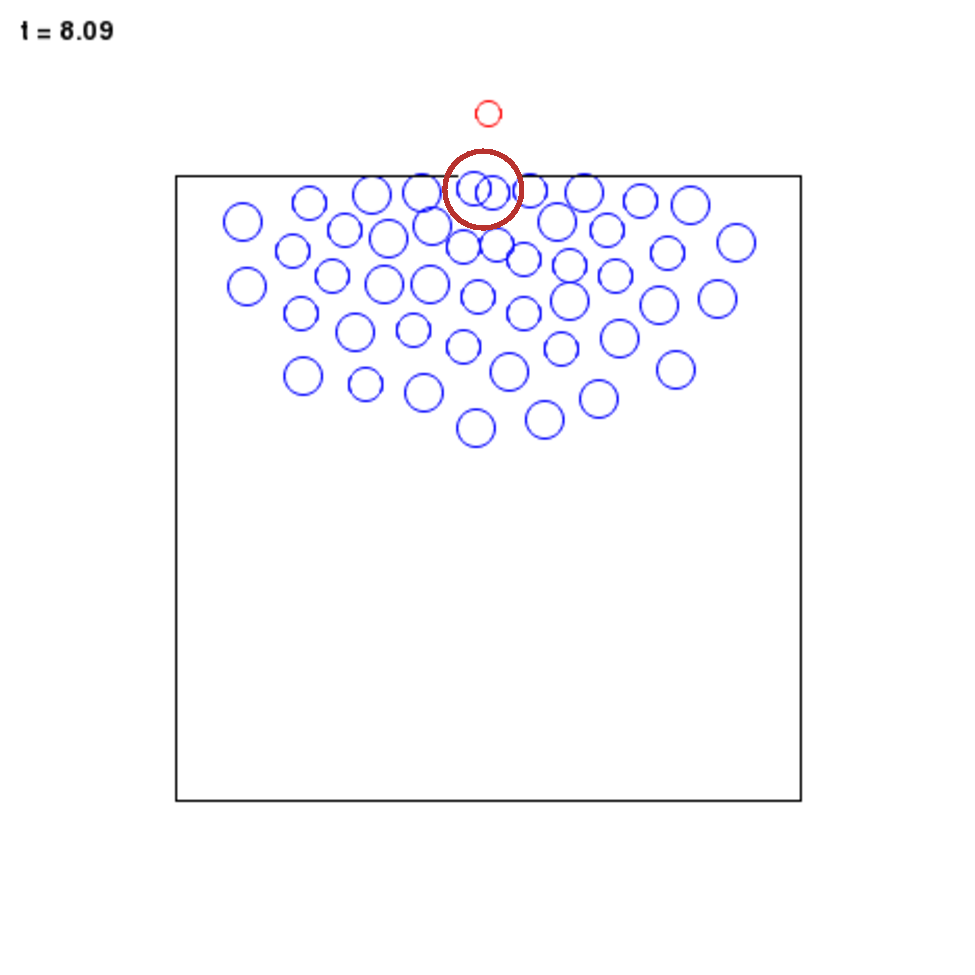
\includegraphics[scale=0.45]{Figures/pedestiranoverlapping.pdf}}
\subfloat[Overlapping between pedestrians and a wall]{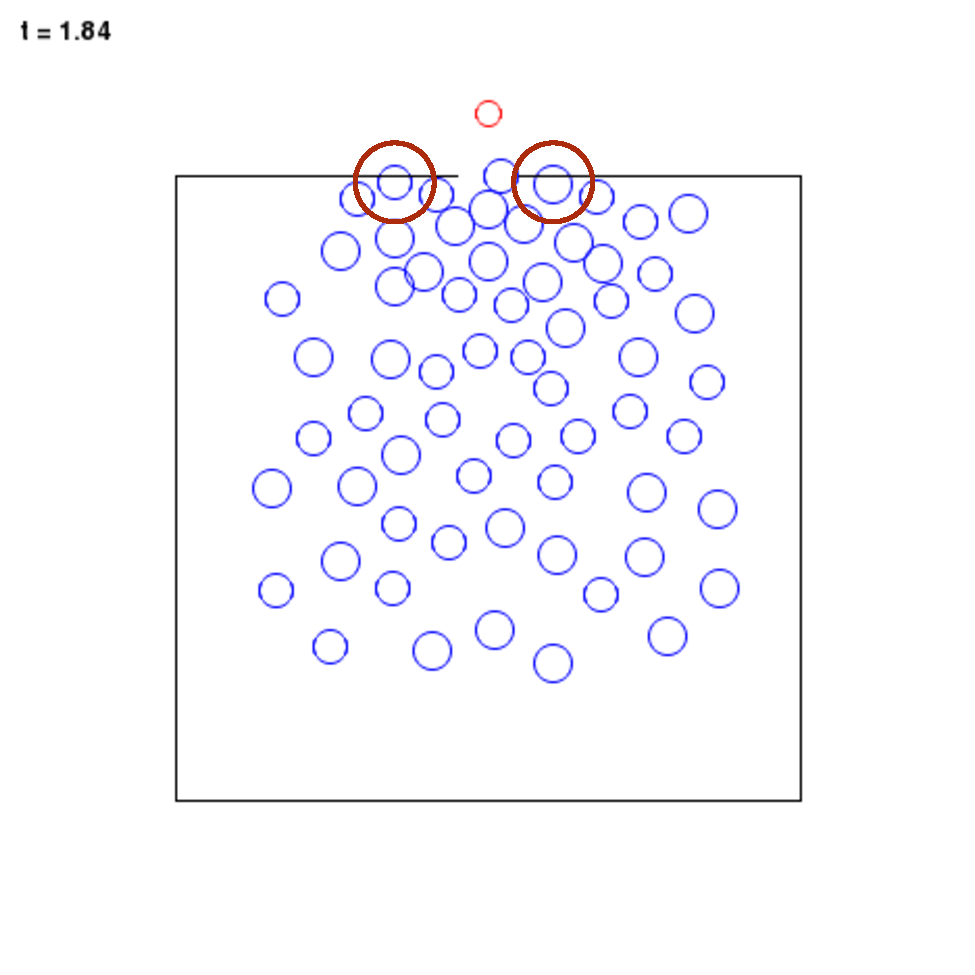
\includegraphics[scale=0.45]{Figures/walloverlapping.pdf}}
\caption{The figure shows two simulations of the squared room. We see the overlapping that can occur between two pedestrians and between the walls and pedestrians. This kind of intersection is seen in most simulations, but they don't cross completely. The red dot on the figures are the desired locations}
\label{fig:overlapping}
\end{figure}

In the figure \ref{fig:overlapping} the overlapping between pedestrians 
themselves and between walls and pedestrians. We see that in some situations 
it is possible for the pedestrians to intersect quite alot, almost reaching 
each others centers. The same thing is seen for the walls, where the wall 
can get quite close to the center of a pedestrians. But inspite of this 
we don't, with the chosen constants, see that they actually do cross. So 
even though it might look like they get sqiuzzed alot together, no completely 
unrealistic situations occur. Also we see no other strange scenarios, like 
people going in a wrong direction or anything like that. So the most basic 
requirements of the model are fulfilled. 

We do however see some unrealistic behavior when we change the values in 
\ref{tbl:parameter-settings} When looking at some of the different phenomenons, 
we need to change certain values like the mean velocity. But when we do 
this it starts to get unrealistic. When raising the desired velocity to 
a speed like $2.5m/s$, we start to see people crossing each other and going 
up to $3.5m/s$ we start to see people crossing the walls. This is a problem 
since these results makes no sence to compares with. Lowering the timestep 
with $1/10$ doesn't change this result at all. So to solve this problem we 
have in some cases raised the wallues of the wall constant $U$ and the 
pedestrains repulsion constant $A$. This makes the repulsions forces 
big enough for the pedestrians to act 'noraml'. We will throughout the 
chapter mention when we change the values and how much it is changed.

\subsection{The phenomena}
In this section we present the results we obtained when we 
tried to replicate the the phenomena reported in our main 
article.

\subsubsection{The faster-is-slower effect}
The faster-is-slower was expected to be seen in the square room scenario.
To see if this effects occurs we have looked at the leaving time as a function 
of the desired velocity of the pedestrains. We made simulations with a desired velocity
going from $1.5m/s$ to $5m/s$ with steps of 0.1. The results are presented in figure 
\ref{fig:isfasterslower}. We see some fluctutation on the graph, but the overall picture 
of the leaving time decreasing when the desired velocity goes up is clear. So there no sign of an increase of 
the leaving time and therefore no faster is slower. The only thing we see is that the negative slope is decreasing, meaning
 that if the pedestrians moves twice as fast, they don't clear the room in half the time. 

%TODO: We should make runs with the desired velcity. This is what they compare with in the letters to nature article. 
% In all the corridor 
%cases (i.e. normal corridor, bottleneck and corridor with free space) 
%we look at how the flow rate at the end of the corridor is 
%affected by an increasing average velocity. In all the scenarios 
%we look at mean velocities from 1.5 to 5 with steps of 0.5. The 
%results are presented in figure \ref{fig:isfasterslower}.

\begin{figure}[h]
\centering
\subfloat[Attempt to see the faster-is-slower effect in the square room.]{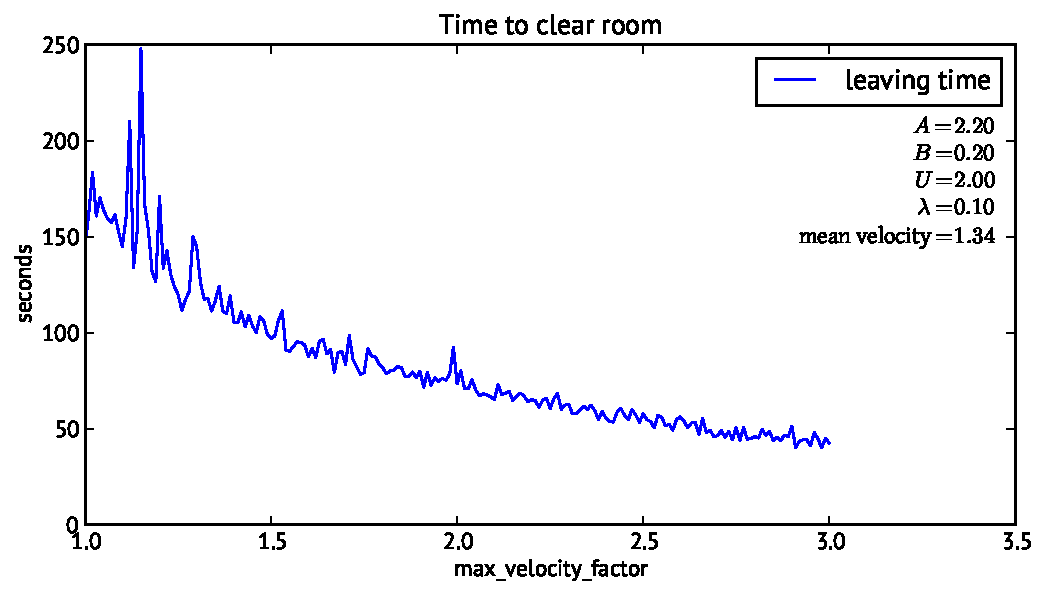
\includegraphics[scale=0.45]{Figures/fastIsSlowNot.pdf}}
\subfloat[Attempt to see the faster-is-slower effect in the normal corridor case.]{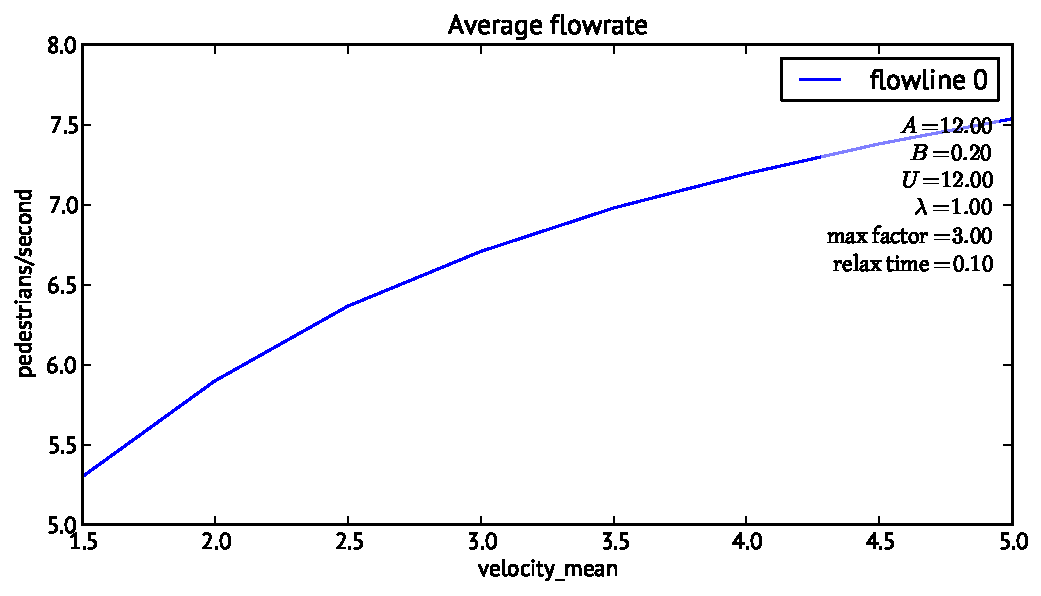
\includegraphics[scale=0.45]{Figures/corridor-flowrate-aggr-velocity_mean.pdf}}\\
\subfloat[Attempt to see the faster-is-slower effect in the bottleneck scenario.]{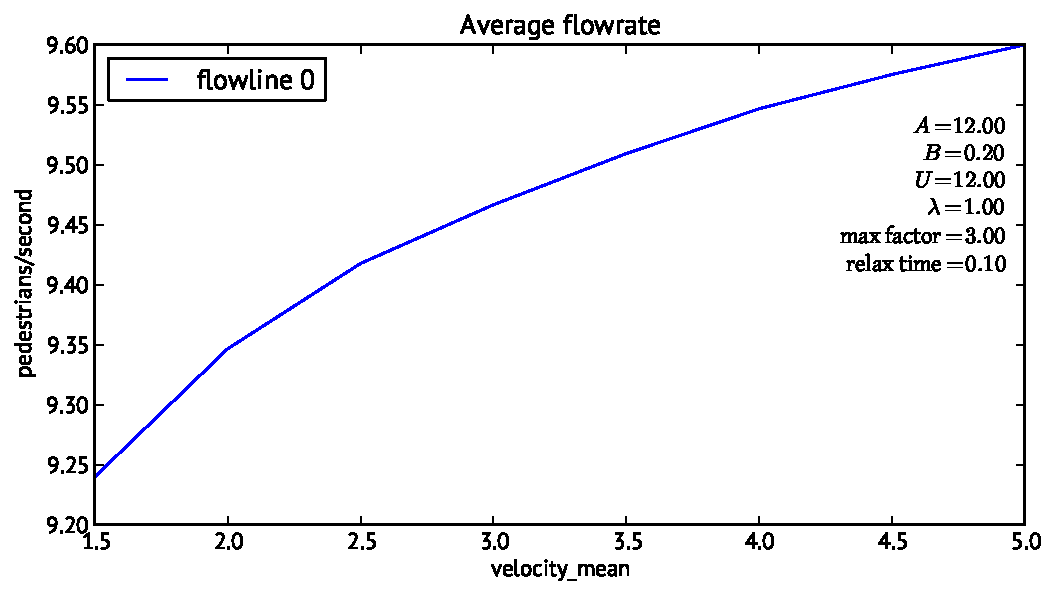
\includegraphics[scale=0.45]{Figures/bottleneck-flowrate-aggr-velocity_mean.pdf}}
\subfloat[Attempt to see the faster-is-slower efffect in the corridor with a wide space.]{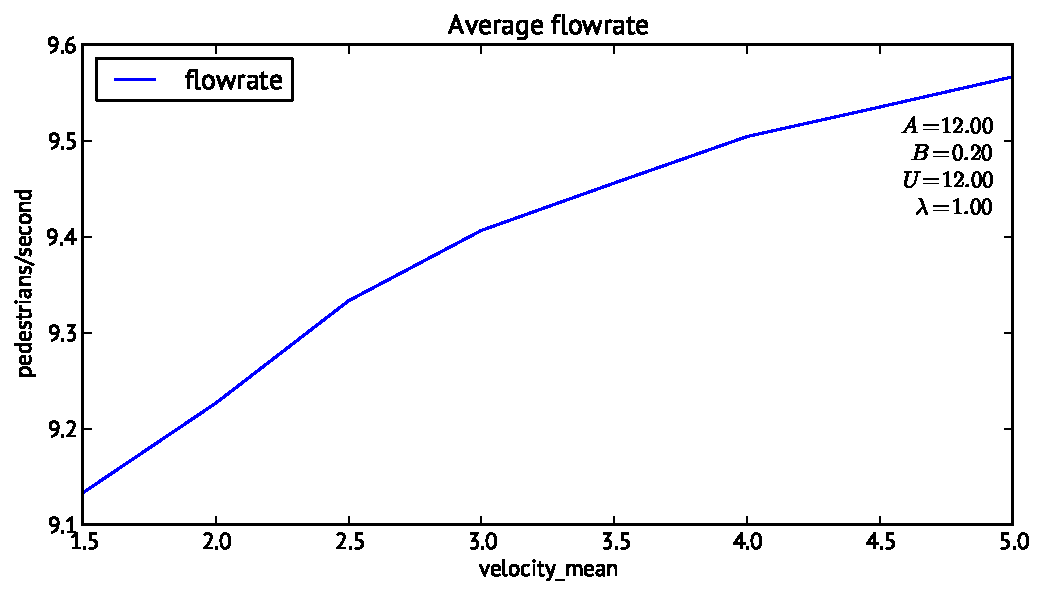
\includegraphics[scale=0.45]{Figures/Wide-kink-one-directional-flowrate-agg.pdf}}
\caption{There is no evidence of the-faster-is slower effect, however it does seem that we see a faster-is-only-slightly-faster effect.}
\label{fig:isfasterslower}
\end{figure}

%We did not observe the faster-is-slower effect in any of our 
%scenarios. However the flow rate does not increase linearly 
%with the average velocity so the interactions between agents 
%and walls does have an effect.

\subsubsection{Freezing by heating effect}
According to \cite{self-org} the freezing by heating effect should 
arise when the max desired velocity of the pedestrians is raised in situations where there is biderectional flow.
We however does not experience this in any of our simulations of the corridor. 
We tried to raise the max velocity, see figure \ref{fig:freezingbyheating1} and figure 
\ref{fig:freezingbyheating05}, but instead of observing the freezing 
by heating effect, we actually saw that the pedestrians got through the corridor 
more easily, and that the density in the corridor was lower when the 
max velocity was high. So like the faster is slower effect again we see no sign of a high desired velocity decreasing/stopping
 the movement of the pedestrians. 

%We think that there are more explations to this 
%result. For the first the pedestrian $\alpha$'s force toward the target
%is higher when $\alpha$'s velocity gets higher, and therefore he more 
%easely pushes his way through the crowd. For the second there are no 
%friction between the pedestrians to slow $\alpha$ speed down, besides 
%the social sphere.

\subsubsection{Lane formation}
Lane formation was expected to happen in the case of bidirectional 
flow in corridors. In our main article you see the following statement:

\begin{quote}
If pedestrians crowds moving in opposite directions meet each other, 
they form small \emph{channels} in the beginning, but these channels 
later merge to produce wide lanes
\end{quote}

Since we have three different corridor cases we have 
looked for lane formation in all of them. The results are presented in 
figure \ref{fig:laneformation}

\begin{figure}[h]
\centering
\subfloat[]{\resizebox{5cm}{!}{\begin{tikzpicture}
\draw[color=blue] (-11.94,-0.70) circle (0.30);
\draw[color=blue] (-9.82,-0.57) circle (0.32);
\draw[color=blue] (-11.22,-0.34) circle (0.32);
\draw[color=green] (11.09,-0.11) circle (0.32);
\draw[color=blue] (-9.11,0.43) circle (0.29);
\draw[color=green] (11.88,0.67) circle (0.30);
\draw[color=green] (9.00,-0.80) circle (0.31);
\draw[color=green] (9.01,0.08) circle (0.31);
\draw[color=blue] (-7.29,0.15) circle (0.30);
\draw[color=green] (10.93,0.72) circle (0.30);
\draw[color=green] (5.10,-0.35) circle (0.29);
\draw[color=green] (9.87,0.45) circle (0.30);
\draw[color=blue] (-6.35,0.41) circle (0.31);
\draw[color=green] (8.28,-0.05) circle (0.29);
\draw[color=blue] (-6.49,-0.16) circle (0.29);
\draw[color=green] (7.18,-0.03) circle (0.29);
\draw[color=green] (5.81,0.46) circle (0.31);
\draw[color=blue] (-3.87,1.03) circle (0.30);
\draw[color=green] (4.40,0.20) circle (0.29);
\draw[color=blue] (-5.52,0.19) circle (0.30);
\draw[color=blue] (-4.49,0.13) circle (0.32);
\draw[color=blue] (-3.03,0.83) circle (0.29);
\draw[color=green] (2.10,-0.22) circle (0.29);
\draw[color=green] (4.29,-0.44) circle (0.30);
\draw[color=green] (-0.75,-0.92) circle (0.29);
\draw[color=blue] (-1.64,0.88) circle (0.30);
\draw[color=green] (-4.81,1.45) circle (0.31);
\draw[color=green] (0.49,-0.94) circle (0.29);
\draw[color=blue] (-0.86,0.86) circle (0.30);
\draw[color=blue] (1.00,-1.15) circle (0.31);
\draw[color=blue] (0.30,0.92) circle (0.29);
\draw[color=green] (-2.08,-0.88) circle (0.29);
\draw[color=blue] (1.92,0.93) circle (0.31);
\draw[color=green] (-2.91,-0.88) circle (0.31);
\draw[color=blue] (4.35,-1.04) circle (0.31);
\draw[color=blue] (2.39,-1.36) circle (0.29);
\draw[color=green] (-7.00,-1.12) circle (0.29);
\draw[color=green] (-3.92,-0.85) circle (0.30);
\draw[color=blue] (8.45,-1.62) circle (0.30);
\draw[color=green] (-5.33,-0.58) circle (0.29);
\draw[color=green] (-6.73,1.07) circle (0.31);
\draw[color=green] (-7.38,0.09) circle (0.29);
\draw[color=green] (-5.80,-1.15) circle (0.29);
\draw[color=green] (-8.17,-1.16) circle (0.29);
\draw[color=green] (-7.53,1.53) circle (0.30);
\draw[color=green] (-8.38,1.54) circle (0.31);
\draw[color=green] (-9.68,0.19) circle (0.31);
\draw[color=green] (-9.13,1.25) circle (0.32);
\draw[color=blue] (8.92,1.27) circle (0.30);
\draw[color=green] (-9.44,0.69) circle (0.31);
\draw[color=green] (-9.52,-1.64) circle (0.31);
\node at (-12.50, 5.83) {t = 20.44};
\useasboundingbox (-12.50, -5.83) rectangle (12.50, 5.83);
\draw[color=black] (-10.00,2.00) -- (10.00,2.00);
\draw[color=black] (-10.00,-2.00) -- (10.00,-2.00);
\end{tikzpicture}
}}
\subfloat[]{\resizebox{5cm}{!}{\begin{tikzpicture}
\draw[color=green] (4.75,-0.01) circle (0.20);
\draw[color=green] (12.34,-0.76) circle (0.19);
\draw[color=green] (11.21,-0.81) circle (0.19);
\draw[color=green] (8.65,0.38) circle (0.21);
\draw[color=blue] (-9.29,-0.26) circle (0.18);
\draw[color=green] (7.46,-0.47) circle (0.20);
\draw[color=green] (5.35,0.05) circle (0.19);
\draw[color=blue] (-4.40,-0.48) circle (0.20);
\draw[color=green] (10.75,0.50) circle (0.20);
\draw[color=green] (6.45,0.55) circle (0.19);
\draw[color=green] (11.25,-0.22) circle (0.21);
\draw[color=green] (11.83,0.88) circle (0.21);
\draw[color=blue] (-8.56,-0.30) circle (0.20);
\draw[color=green] (10.39,0.21) circle (0.20);
\draw[color=green] (12.32,-0.13) circle (0.22);
\draw[color=blue] (-12.30,0.42) circle (0.20);
\draw[color=blue] (-12.39,-0.69) circle (0.21);
\draw[color=green] (11.40,0.38) circle (0.18);
\draw[color=blue] (-10.41,-0.20) circle (0.20);
\draw[color=green] (-3.09,-0.32) circle (0.21);
\draw[color=green] (10.10,-0.32) circle (0.19);
\draw[color=blue] (-2.75,-0.62) circle (0.20);
\draw[color=green] (8.57,-0.53) circle (0.21);
\draw[color=green] (7.06,-0.39) circle (0.19);
\draw[color=green] (8.31,0.36) circle (0.21);
\draw[color=blue] (-7.95,-0.29) circle (0.21);
\draw[color=blue] (-3.92,-0.72) circle (0.20);
\draw[color=green] (6.48,-0.44) circle (0.20);
\draw[color=blue] (-6.86,-0.25) circle (0.21);
\draw[color=blue] (-2.79,-1.32) circle (0.20);
\draw[color=green] (5.45,0.56) circle (0.19);
\draw[color=green] (7.91,0.37) circle (0.19);
\draw[color=blue] (-6.24,-0.31) circle (0.20);
\draw[color=blue] (-11.92,-0.42) circle (0.20);
\draw[color=blue] (1.98,-1.19) circle (0.20);
\draw[color=green] (4.53,0.26) circle (0.20);
\draw[color=green] (1.87,1.69) circle (0.19);
\draw[color=blue] (-5.58,-0.38) circle (0.20);
\draw[color=green] (10.12,0.45) circle (0.19);
\draw[color=green] (0.92,0.17) circle (0.19);
\draw[color=blue] (-3.63,-1.05) circle (0.18);
\draw[color=blue] (-2.23,-0.90) circle (0.18);
\draw[color=green] (1.41,-0.08) circle (0.20);
\draw[color=blue] (-5.13,-0.28) circle (0.22);
\draw[color=blue] (-0.43,-0.83) circle (0.21);
\draw[color=green] (4.15,0.42) circle (0.21);
\draw[color=green] (4.98,0.50) circle (0.21);
\draw[color=green] (0.94,1.03) circle (0.19);
\draw[color=blue] (5.62,0.41) circle (0.21);
\draw[color=green] (3.73,0.98) circle (0.22);
\draw[color=green] (2.20,1.02) circle (0.20);
\draw[color=blue] (0.21,-1.37) circle (0.19);
\draw[color=green] (3.62,0.39) circle (0.21);
\draw[color=green] (0.49,0.26) circle (0.23);
\draw[color=green] (-0.82,0.79) circle (0.19);
\draw[color=blue] (1.17,0.50) circle (0.19);
\draw[color=green] (-0.03,0.74) circle (0.20);
\draw[color=green] (-1.42,1.20) circle (0.21);
\draw[color=green] (-1.36,-0.05) circle (0.20);
\draw[color=blue] (4.64,-0.40) circle (0.18);
\draw[color=green] (0.25,-0.18) circle (0.19);
\draw[color=blue] (0.04,-0.68) circle (0.21);
\draw[color=green] (-4.25,0.54) circle (0.19);
\draw[color=blue] (2.29,-0.47) circle (0.19);
\draw[color=green] (-1.50,0.54) circle (0.20);
\draw[color=blue] (0.75,-0.57) circle (0.20);
\draw[color=green] (-4.44,0.15) circle (0.20);
\draw[color=blue] (5.75,0.14) circle (0.18);
\draw[color=green] (-4.92,0.43) circle (0.20);
\draw[color=green] (-2.17,0.39) circle (0.21);
\draw[color=blue] (3.75,-0.52) circle (0.18);
\draw[color=green] (-5.23,0.16) circle (0.18);
\draw[color=blue] (5.04,-0.41) circle (0.21);
\draw[color=blue] (6.11,0.23) circle (0.19);
\draw[color=green] (-5.90,0.23) circle (0.20);
\draw[color=blue] (6.37,0.07) circle (0.20);
\draw[color=green] (-6.88,0.24) circle (0.20);
\draw[color=blue] (5.47,-0.28) circle (0.20);
\draw[color=blue] (6.88,0.11) circle (0.20);
\draw[color=blue] (8.59,-0.23) circle (0.21);
\draw[color=blue] (7.39,-0.09) circle (0.21);
\draw[color=green] (-7.33,0.27) circle (0.20);
\draw[color=green] (-8.01,0.25) circle (0.21);
\draw[color=blue] (7.82,-0.08) circle (0.19);
\draw[color=green] (-8.59,0.24) circle (0.18);
\draw[color=blue] (9.01,-0.42) circle (0.19);
\draw[color=blue] (8.81,0.21) circle (0.22);
\draw[color=blue] (9.49,0.11) circle (0.20);
\draw[color=green] (-9.29,0.42) circle (0.19);
%\node at (-12.50, 5.83) {t = 40.31};
\useasboundingbox (-12.50, -5.83) rectangle (12.50, 5.83);
\draw[color=black] (-10.00,0.70) -- (-5.00,0.70);
\draw[color=black] (-10.00,-0.70) -- (-5.00,-0.70);
\draw[color=black] (-5.00,0.70) -- (0.00,3.00);
\draw[color=black] (-5.00,-0.70) -- (0.00,-3.00);
\draw[color=black] (0.00,3.00) -- (5.00,0.70);
\draw[color=black] (0.00,-3.00) -- (5.00,-0.70);
\draw[color=black] (5.00,0.70) -- (10.00,0.70);
\draw[color=black] (5.00,-0.70) -- (10.00,-0.70);
\end{tikzpicture}
}}
\subfloat[]{\resizebox{5cm}{!}{\begin{tikzpicture}
\draw[color=blue] (-10.40,-2.20) circle (0.21);
\draw[color=blue] (-10.67,2.32) circle (0.21);
\draw[color=blue] (-8.35,-1.16) circle (0.20);
\draw[color=blue] (-9.80,1.77) circle (0.20);
\draw[color=blue] (-3.11,-0.10) circle (0.20);
\draw[color=blue] (-11.85,-1.75) circle (0.20);
\draw[color=green] (10.98,-0.03) circle (0.18);
\draw[color=green] (7.38,-0.02) circle (0.21);
\draw[color=blue] (-11.85,-2.52) circle (0.21);
\draw[color=green] (9.60,1.13) circle (0.20);
\draw[color=blue] (-10.95,1.44) circle (0.20);
\draw[color=green] (6.79,0.39) circle (0.21);
\draw[color=blue] (-10.94,-1.33) circle (0.19);
\draw[color=blue] (-11.61,-1.14) circle (0.21);
\draw[color=blue] (0.55,-0.24) circle (0.20);
\draw[color=green] (10.79,-0.89) circle (0.20);
\draw[color=green] (12.36,-0.46) circle (0.20);
\draw[color=blue] (-4.86,-1.29) circle (0.20);
\draw[color=green] (2.23,-0.39) circle (0.20);
\draw[color=blue] (-4.15,1.02) circle (0.19);
\draw[color=green] (10.02,-0.88) circle (0.20);
\draw[color=green] (8.10,0.06) circle (0.20);
\draw[color=green] (11.74,-0.57) circle (0.20);
\draw[color=blue] (-9.73,-1.07) circle (0.18);
\draw[color=blue] (-5.50,-1.21) circle (0.19);
\draw[color=green] (7.83,0.07) circle (0.18);
\draw[color=green] (9.23,0.64) circle (0.20);
\draw[color=blue] (-10.34,-1.48) circle (0.19);
\draw[color=green] (8.41,-0.71) circle (0.21);
\draw[color=blue] (-10.95,-0.54) circle (0.19);
\draw[color=blue] (-9.29,-1.37) circle (0.21);
\draw[color=green] (-1.68,-0.20) circle (0.19);
\draw[color=blue] (0.96,0.13) circle (0.22);
\draw[color=green] (7.16,-0.56) circle (0.20);
\draw[color=green] (-0.47,-0.37) circle (0.18);
\draw[color=green] (8.45,0.66) circle (0.19);
\draw[color=blue] (-3.60,0.24) circle (0.20);
\draw[color=blue] (-8.98,1.79) circle (0.20);
\draw[color=green] (1.13,-0.31) circle (0.19);
\draw[color=blue] (-7.64,-1.17) circle (0.19);
\draw[color=green] (9.46,-0.80) circle (0.20);
\draw[color=blue] (-4.44,-0.15) circle (0.21);
\draw[color=blue] (-2.44,0.28) circle (0.21);
\draw[color=blue] (-3.13,0.34) circle (0.19);
\draw[color=green] (3.16,-0.19) circle (0.19);
\draw[color=blue] (-3.76,-0.20) circle (0.21);
\draw[color=green] (-0.66,-0.62) circle (0.19);
\draw[color=green] (-0.09,-0.34) circle (0.21);
\draw[color=green] (1.48,-0.43) circle (0.20);
\draw[color=green] (0.58,0.12) circle (0.20);
\draw[color=blue] (-1.43,-0.26) circle (0.18);
\draw[color=green] (5.83,-0.19) circle (0.19);
\draw[color=blue] (-3.07,-0.54) circle (0.21);
\draw[color=green] (-0.08,0.07) circle (0.19);
\draw[color=green] (-0.98,0.52) circle (0.19);
\draw[color=blue] (0.73,0.36) circle (0.22);
\draw[color=blue] (0.39,0.46) circle (0.21);
\draw[color=blue] (0.16,0.29) circle (0.20);
\draw[color=green] (-1.00,-0.61) circle (0.19);
\draw[color=green] (-0.08,0.36) circle (0.22);
\draw[color=blue] (-1.11,-0.03) circle (0.19);
\draw[color=green] (-0.39,0.31) circle (0.20);
\draw[color=blue] (-1.52,0.16) circle (0.18);
\draw[color=blue] (1.41,-0.07) circle (0.21);
\draw[color=blue] (-2.60,-0.42) circle (0.20);
\draw[color=blue] (-0.72,-0.08) circle (0.20);
\draw[color=blue] (0.78,0.69) circle (0.21);
\draw[color=blue] (2.00,0.55) circle (0.20);
\draw[color=blue] (-0.12,-0.11) circle (0.20);
\draw[color=blue] (0.28,-0.35) circle (0.21);
\draw[color=blue] (1.79,0.16) circle (0.21);
\draw[color=green] (-0.63,0.53) circle (0.20);
\draw[color=blue] (1.26,0.46) circle (0.22);
\draw[color=blue] (0.53,-0.49) circle (0.20);
\draw[color=blue] (0.94,-0.76) circle (0.19);
\draw[color=green] (-1.87,0.78) circle (0.20);
\draw[color=blue] (1.36,-0.83) circle (0.20);
\draw[color=green] (-1.34,0.79) circle (0.18);
\draw[color=blue] (1.17,0.84) circle (0.21);
\draw[color=green] (-2.34,1.04) circle (0.21);
\draw[color=green] (-1.46,-0.83) circle (0.20);
\draw[color=blue] (1.73,-1.02) circle (0.21);
\draw[color=blue] (1.99,-0.68) circle (0.19);
\draw[color=green] (-2.02,-1.10) circle (0.19);
\draw[color=blue] (1.61,0.92) circle (0.19);
\draw[color=green] (-2.82,-0.98) circle (0.19);
\draw[color=green] (-2.93,1.35) circle (0.20);
\draw[color=green] (-3.35,-0.80) circle (0.20);
\draw[color=blue] (2.28,-1.14) circle (0.21);
\draw[color=green] (-3.47,1.47) circle (0.20);
\draw[color=green] (-3.07,0.84) circle (0.21);
\draw[color=blue] (3.21,-1.53) circle (0.20);
\draw[color=green] (-3.86,-0.63) circle (0.18);
\draw[color=blue] (3.62,-1.09) circle (0.19);
\draw[color=green] (-4.29,0.75) circle (0.21);
\draw[color=blue] (2.60,1.19) circle (0.20);
\draw[color=green] (-3.69,0.40) circle (0.19);
\draw[color=green] (-4.62,-0.19) circle (0.19);
\draw[color=blue] (4.28,1.31) circle (0.20);
\draw[color=blue] (4.82,-1.35) circle (0.19);
\draw[color=blue] (5.10,1.27) circle (0.19);
\draw[color=green] (-4.51,1.15) circle (0.20);
\draw[color=green] (-5.94,0.99) circle (0.21);
\draw[color=green] (-4.98,0.42) circle (0.20);
\draw[color=blue] (5.52,-1.40) circle (0.20);
\draw[color=green] (-5.81,-0.13) circle (0.20);
\draw[color=blue] (6.54,1.68) circle (0.19);
\draw[color=blue] (6.17,-1.30) circle (0.20);
\draw[color=green] (-6.91,-0.28) circle (0.20);
\draw[color=blue] (5.85,1.09) circle (0.21);
\draw[color=green] (-6.77,0.58) circle (0.20);
\draw[color=green] (-7.60,1.00) circle (0.21);
\draw[color=blue] (7.17,-1.30) circle (0.19);
\draw[color=blue] (7.72,1.17) circle (0.17);
\draw[color=green] (-7.80,-0.18) circle (0.20);
\draw[color=green] (-8.00,0.41) circle (0.19);
\draw[color=blue] (8.36,0.06) circle (0.18);
\draw[color=blue] (8.85,0.03) circle (0.19);
\draw[color=blue] (8.50,-0.31) circle (0.21);
\draw[color=green] (-8.97,-0.40) circle (0.20);
\draw[color=blue] (9.47,0.59) circle (0.20);
\draw[color=green] (-9.47,-0.62) circle (0.20);
\draw[color=green] (-9.22,0.21) circle (0.19);
\node at (-12.50, 5.83) {t = 43.45};
\useasboundingbox (-12.50, -5.83) rectangle (12.50, 5.83);
\draw[color=black] (-10.00,3.00) -- (-5.00,3.00);
\draw[color=black] (-10.00,-3.00) -- (-5.00,-3.00);
\draw[color=black] (-5.00,3.00) -- (0.00,0.50);
\draw[color=black] (-5.00,-3.00) -- (0.00,-0.50);
\draw[color=black] (0.00,0.50) -- (5.00,3.00);
\draw[color=black] (0.00,-0.50) -- (5.00,-3.00);
\draw[color=black] (5.00,3.00) -- (10.00,3.00);
\draw[color=black] (5.00,-3.00) -- (10.00,-3.00);
\end{tikzpicture}
}}
\caption{Lane formation in the different corridors.}
\label{fig:laneformation}
\end{figure}

Lane formation is observed in every case.

\subsubsection{The Oscillatory flow}
The oscillatory flow is expected to arise in the case of bidirectional 
flow through a bottleneck. The results are presented in figure
\ref{fig:oscillitoryflow}.

\begin{figure}[h]
\centering
\subfloat[A screen shot of bidirectional flow in the bottlenck]{\resizebox{7cm}{!}{\begin{tikzpicture}
\draw[color=blue] (-10.40,-2.20) circle (0.21);
\draw[color=blue] (-10.67,2.32) circle (0.21);
\draw[color=blue] (-8.35,-1.16) circle (0.20);
\draw[color=blue] (-9.80,1.77) circle (0.20);
\draw[color=blue] (-3.11,-0.10) circle (0.20);
\draw[color=blue] (-11.85,-1.75) circle (0.20);
\draw[color=green] (10.98,-0.03) circle (0.18);
\draw[color=green] (7.38,-0.02) circle (0.21);
\draw[color=blue] (-11.85,-2.52) circle (0.21);
\draw[color=green] (9.60,1.13) circle (0.20);
\draw[color=blue] (-10.95,1.44) circle (0.20);
\draw[color=green] (6.79,0.39) circle (0.21);
\draw[color=blue] (-10.94,-1.33) circle (0.19);
\draw[color=blue] (-11.61,-1.14) circle (0.21);
\draw[color=blue] (0.55,-0.24) circle (0.20);
\draw[color=green] (10.79,-0.89) circle (0.20);
\draw[color=green] (12.36,-0.46) circle (0.20);
\draw[color=blue] (-4.86,-1.29) circle (0.20);
\draw[color=green] (2.23,-0.39) circle (0.20);
\draw[color=blue] (-4.15,1.02) circle (0.19);
\draw[color=green] (10.02,-0.88) circle (0.20);
\draw[color=green] (8.10,0.06) circle (0.20);
\draw[color=green] (11.74,-0.57) circle (0.20);
\draw[color=blue] (-9.73,-1.07) circle (0.18);
\draw[color=blue] (-5.50,-1.21) circle (0.19);
\draw[color=green] (7.83,0.07) circle (0.18);
\draw[color=green] (9.23,0.64) circle (0.20);
\draw[color=blue] (-10.34,-1.48) circle (0.19);
\draw[color=green] (8.41,-0.71) circle (0.21);
\draw[color=blue] (-10.95,-0.54) circle (0.19);
\draw[color=blue] (-9.29,-1.37) circle (0.21);
\draw[color=green] (-1.68,-0.20) circle (0.19);
\draw[color=blue] (0.96,0.13) circle (0.22);
\draw[color=green] (7.16,-0.56) circle (0.20);
\draw[color=green] (-0.47,-0.37) circle (0.18);
\draw[color=green] (8.45,0.66) circle (0.19);
\draw[color=blue] (-3.60,0.24) circle (0.20);
\draw[color=blue] (-8.98,1.79) circle (0.20);
\draw[color=green] (1.13,-0.31) circle (0.19);
\draw[color=blue] (-7.64,-1.17) circle (0.19);
\draw[color=green] (9.46,-0.80) circle (0.20);
\draw[color=blue] (-4.44,-0.15) circle (0.21);
\draw[color=blue] (-2.44,0.28) circle (0.21);
\draw[color=blue] (-3.13,0.34) circle (0.19);
\draw[color=green] (3.16,-0.19) circle (0.19);
\draw[color=blue] (-3.76,-0.20) circle (0.21);
\draw[color=green] (-0.66,-0.62) circle (0.19);
\draw[color=green] (-0.09,-0.34) circle (0.21);
\draw[color=green] (1.48,-0.43) circle (0.20);
\draw[color=green] (0.58,0.12) circle (0.20);
\draw[color=blue] (-1.43,-0.26) circle (0.18);
\draw[color=green] (5.83,-0.19) circle (0.19);
\draw[color=blue] (-3.07,-0.54) circle (0.21);
\draw[color=green] (-0.08,0.07) circle (0.19);
\draw[color=green] (-0.98,0.52) circle (0.19);
\draw[color=blue] (0.73,0.36) circle (0.22);
\draw[color=blue] (0.39,0.46) circle (0.21);
\draw[color=blue] (0.16,0.29) circle (0.20);
\draw[color=green] (-1.00,-0.61) circle (0.19);
\draw[color=green] (-0.08,0.36) circle (0.22);
\draw[color=blue] (-1.11,-0.03) circle (0.19);
\draw[color=green] (-0.39,0.31) circle (0.20);
\draw[color=blue] (-1.52,0.16) circle (0.18);
\draw[color=blue] (1.41,-0.07) circle (0.21);
\draw[color=blue] (-2.60,-0.42) circle (0.20);
\draw[color=blue] (-0.72,-0.08) circle (0.20);
\draw[color=blue] (0.78,0.69) circle (0.21);
\draw[color=blue] (2.00,0.55) circle (0.20);
\draw[color=blue] (-0.12,-0.11) circle (0.20);
\draw[color=blue] (0.28,-0.35) circle (0.21);
\draw[color=blue] (1.79,0.16) circle (0.21);
\draw[color=green] (-0.63,0.53) circle (0.20);
\draw[color=blue] (1.26,0.46) circle (0.22);
\draw[color=blue] (0.53,-0.49) circle (0.20);
\draw[color=blue] (0.94,-0.76) circle (0.19);
\draw[color=green] (-1.87,0.78) circle (0.20);
\draw[color=blue] (1.36,-0.83) circle (0.20);
\draw[color=green] (-1.34,0.79) circle (0.18);
\draw[color=blue] (1.17,0.84) circle (0.21);
\draw[color=green] (-2.34,1.04) circle (0.21);
\draw[color=green] (-1.46,-0.83) circle (0.20);
\draw[color=blue] (1.73,-1.02) circle (0.21);
\draw[color=blue] (1.99,-0.68) circle (0.19);
\draw[color=green] (-2.02,-1.10) circle (0.19);
\draw[color=blue] (1.61,0.92) circle (0.19);
\draw[color=green] (-2.82,-0.98) circle (0.19);
\draw[color=green] (-2.93,1.35) circle (0.20);
\draw[color=green] (-3.35,-0.80) circle (0.20);
\draw[color=blue] (2.28,-1.14) circle (0.21);
\draw[color=green] (-3.47,1.47) circle (0.20);
\draw[color=green] (-3.07,0.84) circle (0.21);
\draw[color=blue] (3.21,-1.53) circle (0.20);
\draw[color=green] (-3.86,-0.63) circle (0.18);
\draw[color=blue] (3.62,-1.09) circle (0.19);
\draw[color=green] (-4.29,0.75) circle (0.21);
\draw[color=blue] (2.60,1.19) circle (0.20);
\draw[color=green] (-3.69,0.40) circle (0.19);
\draw[color=green] (-4.62,-0.19) circle (0.19);
\draw[color=blue] (4.28,1.31) circle (0.20);
\draw[color=blue] (4.82,-1.35) circle (0.19);
\draw[color=blue] (5.10,1.27) circle (0.19);
\draw[color=green] (-4.51,1.15) circle (0.20);
\draw[color=green] (-5.94,0.99) circle (0.21);
\draw[color=green] (-4.98,0.42) circle (0.20);
\draw[color=blue] (5.52,-1.40) circle (0.20);
\draw[color=green] (-5.81,-0.13) circle (0.20);
\draw[color=blue] (6.54,1.68) circle (0.19);
\draw[color=blue] (6.17,-1.30) circle (0.20);
\draw[color=green] (-6.91,-0.28) circle (0.20);
\draw[color=blue] (5.85,1.09) circle (0.21);
\draw[color=green] (-6.77,0.58) circle (0.20);
\draw[color=green] (-7.60,1.00) circle (0.21);
\draw[color=blue] (7.17,-1.30) circle (0.19);
\draw[color=blue] (7.72,1.17) circle (0.17);
\draw[color=green] (-7.80,-0.18) circle (0.20);
\draw[color=green] (-8.00,0.41) circle (0.19);
\draw[color=blue] (8.36,0.06) circle (0.18);
\draw[color=blue] (8.85,0.03) circle (0.19);
\draw[color=blue] (8.50,-0.31) circle (0.21);
\draw[color=green] (-8.97,-0.40) circle (0.20);
\draw[color=blue] (9.47,0.59) circle (0.20);
\draw[color=green] (-9.47,-0.62) circle (0.20);
\draw[color=green] (-9.22,0.21) circle (0.19);
\node at (-12.50, 5.83) {t = 43.45};
\useasboundingbox (-12.50, -5.83) rectangle (12.50, 5.83);
\draw[color=black] (-10.00,3.00) -- (-5.00,3.00);
\draw[color=black] (-10.00,-3.00) -- (-5.00,-3.00);
\draw[color=black] (-5.00,3.00) -- (0.00,0.50);
\draw[color=black] (-5.00,-3.00) -- (0.00,-0.50);
\draw[color=black] (0.00,0.50) -- (5.00,3.00);
\draw[color=black] (0.00,-0.50) -- (5.00,-3.00);
\draw[color=black] (5.00,3.00) -- (10.00,3.00);
\draw[color=black] (5.00,-3.00) -- (10.00,-3.00);
\end{tikzpicture}
}}
\subfloat[Plot of the flow rate beyond each end of the corridor.]{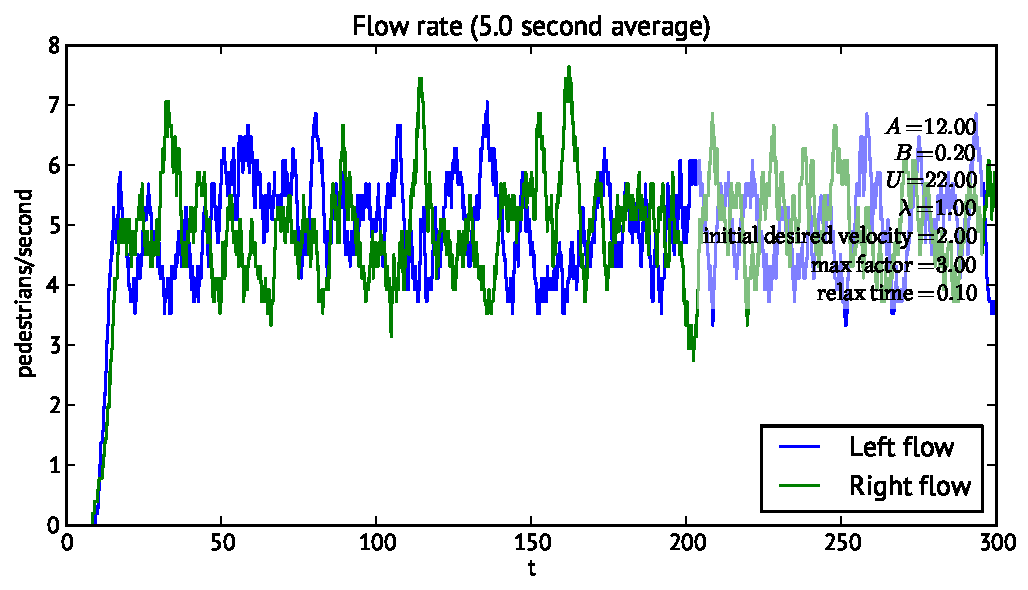
\includegraphics[scale=0.5]{Figures/bottleneck-flowrate-2.pdf}}
\caption{}
\label{fig:oscillitoryflow}
\end{figure}

When looking at the simulation while it is running it is not 
immediately clear that the oscillatory flow occurs. Clogging 
appears in both ends of the bottleneck and people are sometimes 
squeezed through the bottleneck. The graph presented in 
\ref{fig:oscillitoryflow} does indicate that the oscillatory 
flow occurs to some extent.

% \subsection{The square room scenario}
% In this scenario we simulate pedestrians leaving a square room of 10 m by 
% 10 m with a single $80cm$ wide door. 100 pedestrians are positioned randomly 
% throughout the room. The second the simulation start all pedestrians head 
% for the exit. The parameters for this simulation are as in 
% \ref{tbl:parameter-settings}
% 
% First the claim of the "faster-is-slower" effect is tested.
% \begin{quote}
% Even counterintuitive
% effects are well reproduced. This includes the “faster is-
% slower effect” and stripe formation in intersecting flows. \cite{self-org}
% \end{quote}
% We would then expect that a high nervousness would lead to slower evacuation, because of additional clogging at the doorway. But this phenomena do not occur in our simulation see figure \ref{FastIsSlow}
% \begin{figure}
% \centering
% 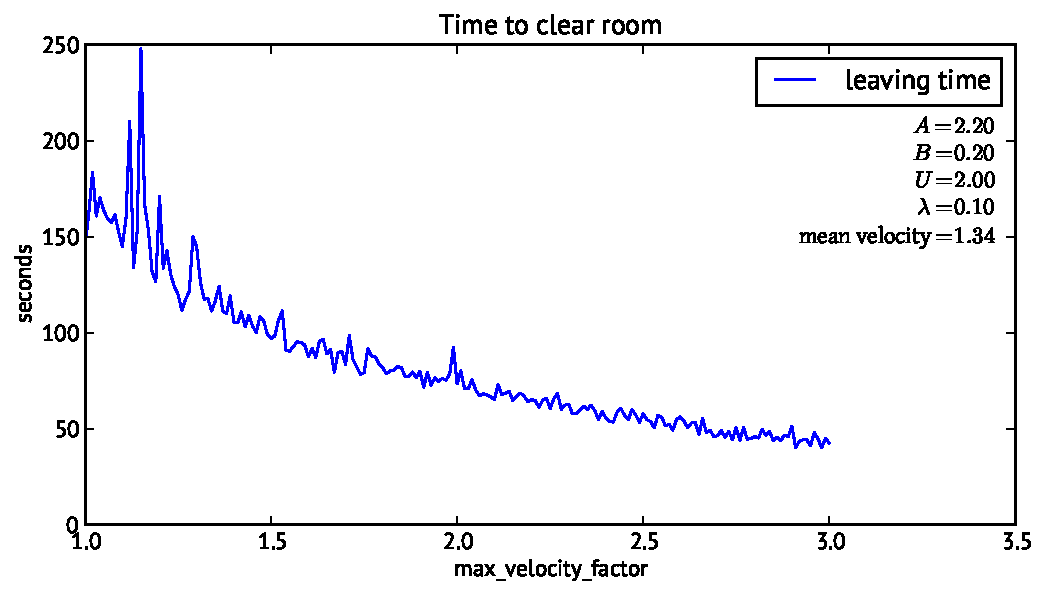
\includegraphics[scale=0.5]{Figures/fastIsSlowNot}
% \caption{Fast is not slow}
% \label{FastIsSlow}
% \end{figure}
% 
% The larger the nervousness the faster is the evacuation. We have increased 
% the max-velocity factor sow much that people eventually move through the walls. 
% This start occurring around max-velocity-factor = 2.5, and measurements beyond 
% this point are neglected.
% 
% Pedestrian flow rate is measure in the door opening, and the density of pedestrians 
% in a 2 m by 2 m area directly in front of the door is measured. We also measure 
% the time it takes for all pedestrians to leave the room.
% 
% The parameters for this simulation are the ones shown in 
% \ref{tbl:parameter-settings}
% 
% % TODO: Add parameters that are varied.
% 
% 
% \subsection{The corridor scenario}
% In this scenario we simulate pedestrians walking in both directions along a 20 
% m long and six metres wide corridor. The pedestrians are divided into two 
% groups, starting in opposite ends of the corridor and moving towards each 
% other. The targets the pedestrians move towards are set 500 metres to each 
% side, to make pedestrians walk in almost a straight line instead of converging 
% towards the middle of the corridor. Flow rate is measured in the middle of the 
% corridor, as is density. We start out with 100 pedestrians, adding a 
% continuous inflow of three pedestrians per second, to simulate people arriving 
% from outside the simulated area. Both the initial placement and the inflow of 
% pedestrians are distributed randomly (i.e. approximately evenly) between the 
% two ends of the corridor.
% 
% We expect to see lane formations through out our simulations
% and the freezing by heating effect when we start raising the mean velocity
% of the agents.
% 
% \subsubsection{Intial conditions and relaxation time $1,0$ second}
% 
% The parameters for this simulation are as in \ref{tbl:parameter-settings} with the exception of the pedestrians
% \begin{itemize*}
%     \item Number of pedestrians: $40$ starting, adding $3/s$.
% \end{itemize*}
% 
% When running the simulation we observe lane formations, and they almost clog up
% in the corridor.
% 
% When we do a simulation with the max velocity factor set to $4.0$, instead 
% of the normal $1.3$, the clogging that occurs in the beginning eases up, 
% and the pedestrians relatively fast get out of the clogging and continuous 
% toward their target. In this simulation we also observe lane formations.
% 
% \begin{figure}[h]
% \centering
% \subfloat[The figure show the density in corridor when the parameters are set as \cite{ABconstant} and \cite{self-org}.]{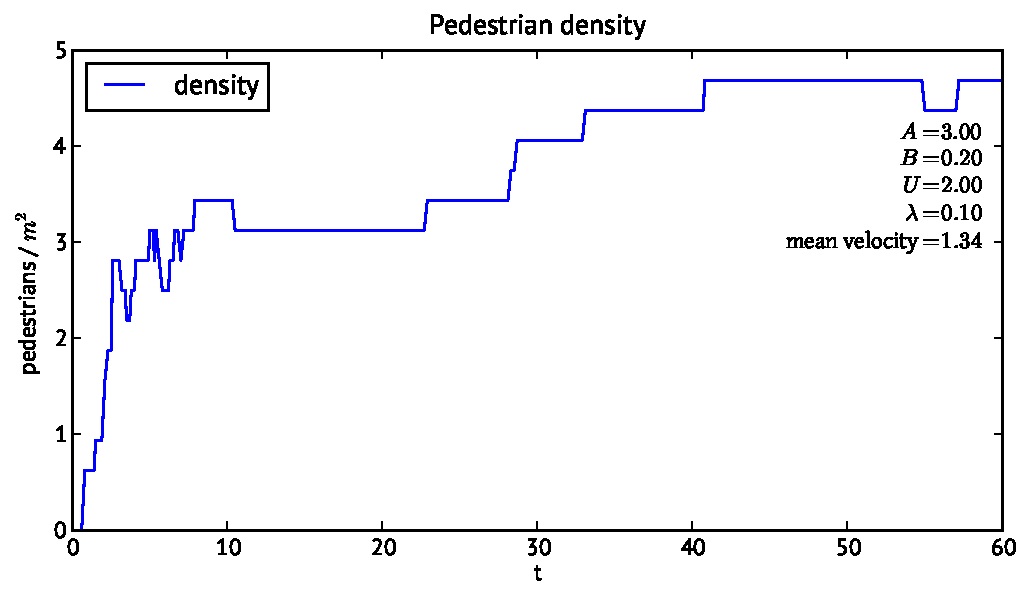
\includegraphics[scale=0.45]{Figures/dens_init_relax1.pdf}}
% \subfloat[This figure shows the density in the corridor when the max velocity factor is set to $4.0$, and the other parameters as figure a.]{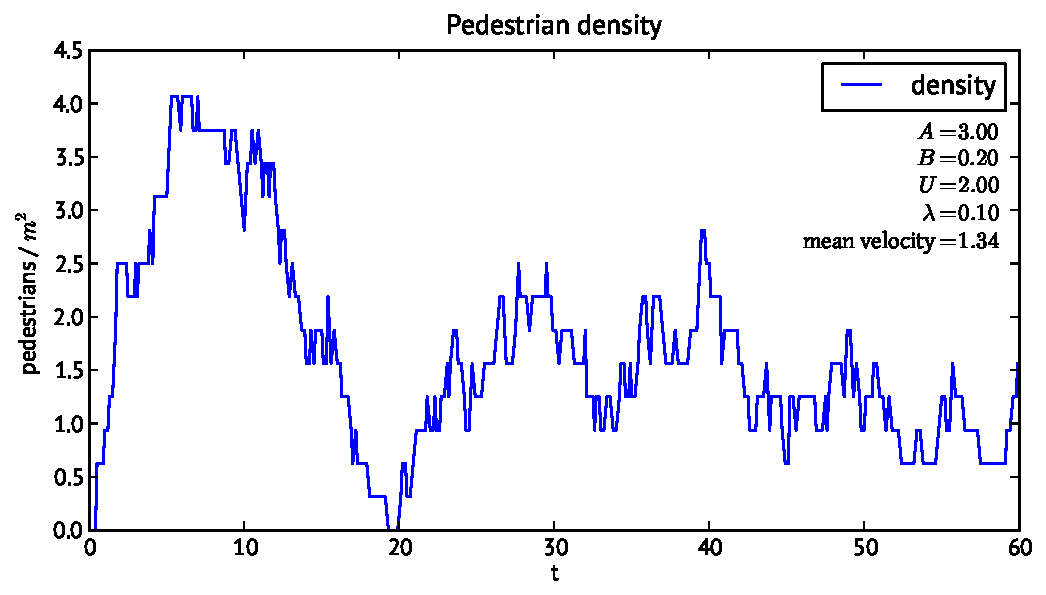
\includegraphics[scale=0.45]{Figures/dens_mvel4_relax1.pdf}}
% \caption{These figures was made to see if the freezing by heating effect when raising the max velocity factor. As seen in the figures, the
% density does not increase when the max desired velocity is increased. When raising the max desired velocity the density gets lower because
% the pedestrians more easely get through the crowd.}
% \label{fig:freezingbyheating1}
% \end{figure}
% 
% \subsubsection{Intial conditions and relaxation time $0,5$ second}
% \cite{helbing00} set the relaxation time to $0,5$. As the first corridor simulations we set the parameters as \cite{ABconstant}
% and then change the relaxation time to $0,5$ as \cite{helbing00}. After the simulation with the initial conditions, we raise the
% max desired velocity to see if we can replicate the freezing by heating effect.
% 
% The initial simulation has the values from \ref{tbl:parameter-settings} with the exceptions:
% 
% \begin{itemize*}
%     \item Relaxation time: $0,5 s$.
%     \item Number of pedestrians: $40$ starting, adding $3/s$.
% \end{itemize*}
% 
% The next simulation we keep the new relaxation time, but changes the max velocity factor set to $4.0$
% 
% 
% When comparing the simulations we do not see the freezing by heating effect.
% Instead we see that the pedestrians more easely escape the clogging, and the 
% flow in each directionsgets more steady. In both simulations we observed lane 
% formation.
% 
% \begin{figure}[h]
% \centering
% \subfloat[The figure show the density in corridor when the parameters are set as \cite{ABconstant} and \cite{helbing00}.]{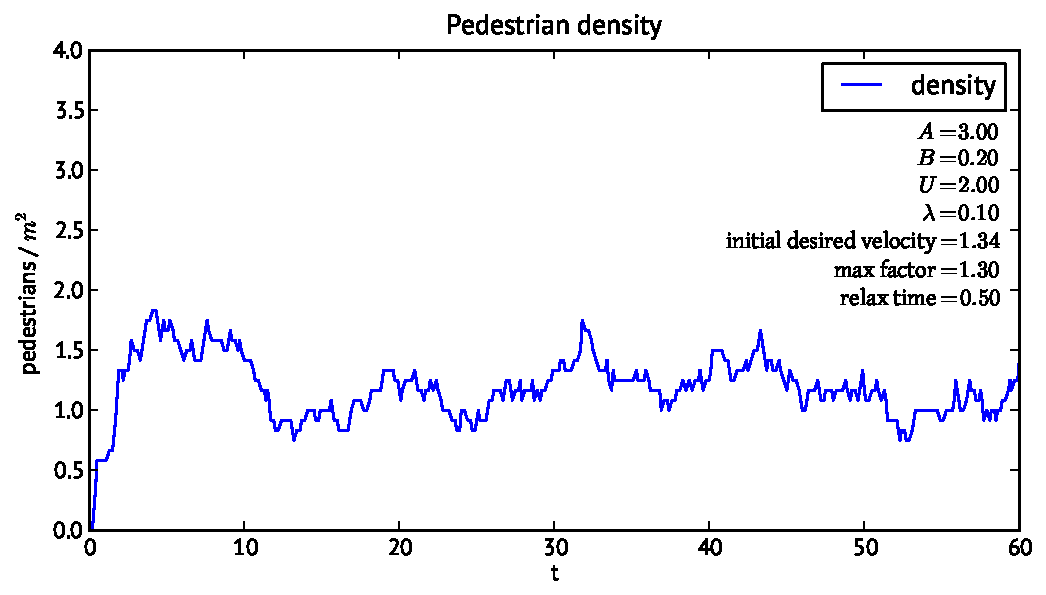
\includegraphics[scale=0.45]{Figures/dens_init_relax05.pdf}}
% \subfloat[This figure shows the density in the corridor when the max velocity factor is set to $4.0$ and the max desired velocity is set to $4,0$, and the other parameters as figure a.]{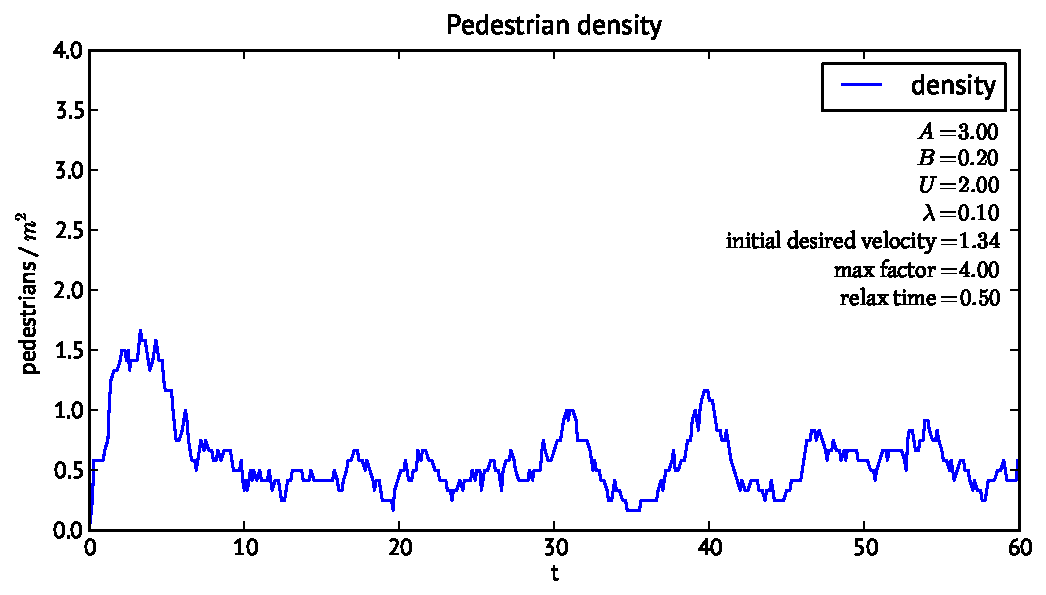
\includegraphics[scale=0.45]{Figures/dens_mvel4_relax05.pdf}}
% \caption{These figures was made to see if the freezing by heating effect when raising the max velocity factor. As seen in the figures, the
% density does not increase when the max desired velocity is increased. When raising the max desired velocity the density gets lower because
% the pedestrians more easely get through the crowd. The difference between figure \ref{fig:freezingbyheating1} and this is the relation time,
% respectively $1,0$ and $0,5$.}
% \label{fig:freezingbyheating05}
% \end{figure}
% 
% \subsubsection{Comparison between the relaxation time $1,0$ second and $0,5$ second}
% When simulating the corridor with the initial conditions and changing 
% the relaxation time from $1,0 s$ to $0,5 s$, the pedestrians do not get 
% stuck as easely when the relaxtion time is $0,5 s$ as they do when the 
% relaxation time is $1,0 s$. This can be seen in figure 
% \ref{fig:comparison_of_timestep}, that in (a), the density get high faster, 
% while in (b) the density does not increase as fast as (a). When the 
% relaxation time is $0,5 s$, the pedestrians reacts faster, in the sense 
% that they speed up faster, after collisions with pedestrians walking in 
% the other direction.
% 
% \begin{figure}[h]
% \centering
% \subfloat[The figure show the density in corridor when the relaxation time is set to $1,0 s$]{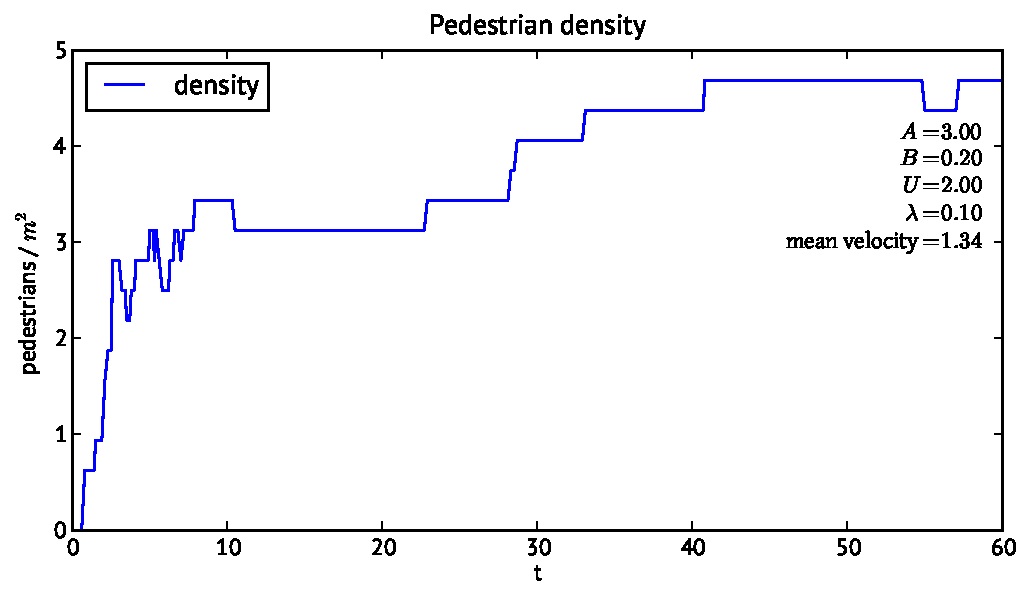
\includegraphics[scale=0.45]{Figures/dens_init_relax1.pdf}}
% \subfloat[This figure shows the density in the corridor when the relaxation time is set to $0,5 s$]{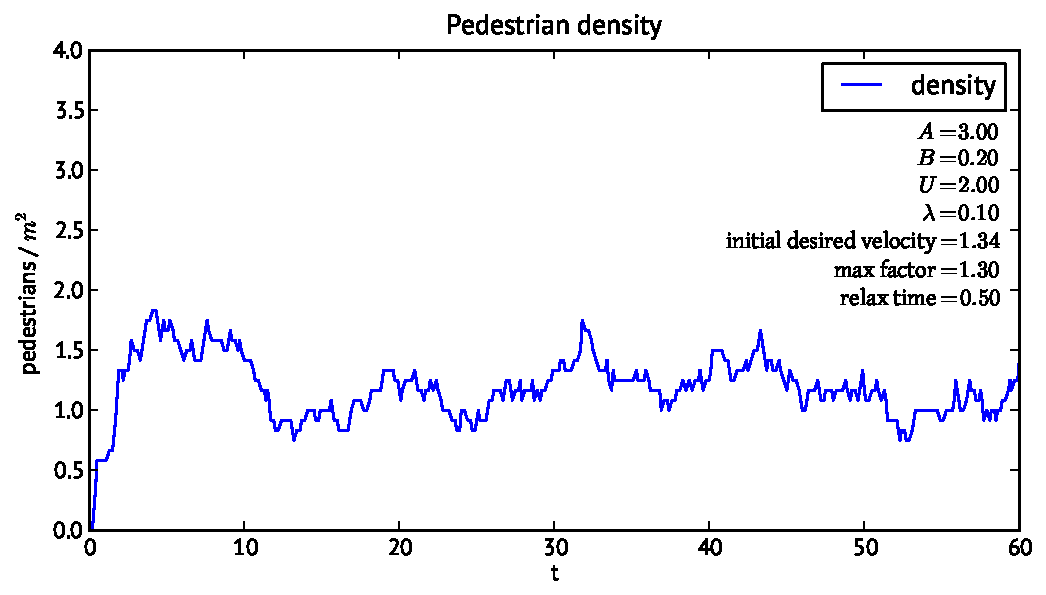
\includegraphics[scale=0.45]{Figures/dens_init_relax05.pdf}}
% \caption{These figures show the difference of the density when changing the relaxation time of the model from $1,0 s$ to $0,5 s$.
% It is seen the the density is more steady when the relaxtion time is $0,5 s$ instead of $1,0 s$}
% \label{fig:comparison_of_timestep}
% \end{figure}
% 
% A possible explanation of why the density is more steady through out 
% the simulation when the relaxation time is $0,5 s$, is that the 
% pedestrians reacts faster to changes of their velocity. Thus when they 
% bump into each other, they speed up faster, and therefore avoid 
% clogging up before more get in their path.
% 
% \subsubsection{Freezing by heating effect}
% According to \cite{self-org} the freezing by heating effect should 
% arise when the max desired velocity of the pedestrians was raised.
% That is that clogging should arise when raising the max velocity of 
% the pedestrians, because more are ariving to the possible clogging area, 
% and thus have more trouble getting through the crowd. We tried to raise 
% the max velocity, see figure \ref{fig:freezingbyheating1} and figure 
% \ref{fig:freezingbyheating05}, but instead of observing the freezing 
% by heating effect, we saw that the pedestrians got through the corridor 
% more easely, and that the density in the corridor was lower when the 
% max velocity was high. We think that there are more explations to this 
% result. For the first the pedestrian $\alpha$'s force toward the target
% is higher when $\alpha$'s velocity gets higher, and therefore he more 
% easely pushes his way through the crowd. For the second there are no 
% friction between the pedestrians to slow $\alpha$ speed down, besides 
% the social sphere.
% 
% \subsection{The bottleneck}
% In this scenario we wanted to the the oscillitory flows that is reported 
% in \cite{self-org} to happen when you have a bidirectional flaw through a 
% bottleneck.
% 
% \subsubsection{The Oscillitory flow}
% 
% \begin{figure}[h]
% \centering
% {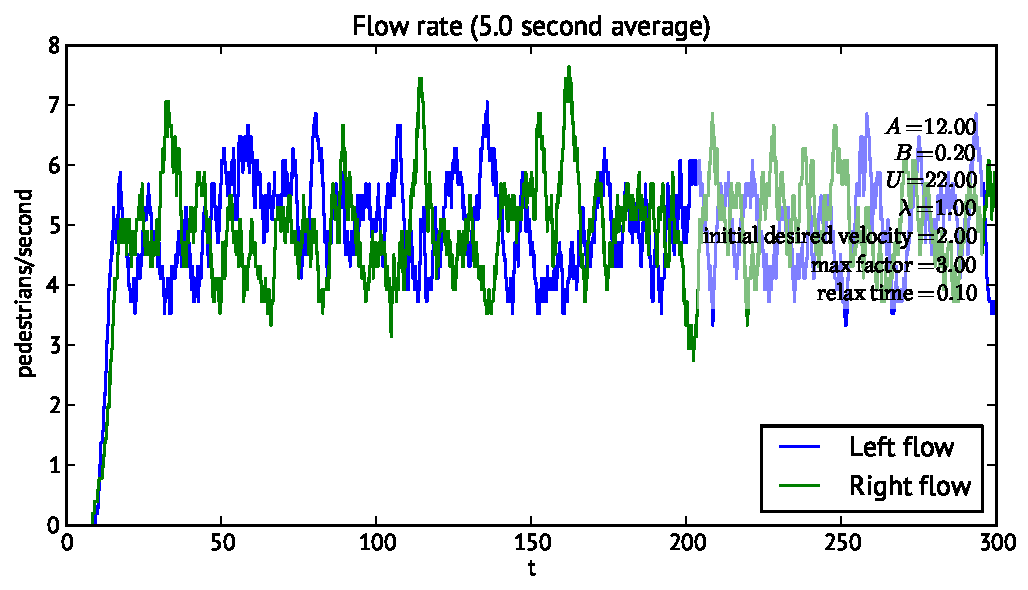
\includegraphics[scale=0.5]{Figures/bottleneck-flowrate-2.pdf}}
% \caption{A screen shot of the bottleneck simulation.}
% \label{fig:oscillitoryflow}
% \end{figure}
% 
% \subsection{The corridor with open space}
% In this scenario we wanted to reproduce the results that people start to 
% clock up in a corridor if there is a sudden area that allow pedestrians to try 
% and overtake each other. To see if the flow rate is affected by the pedestrians 
% who try to overtake each other we compare the flow rate with the wide space with 
% the flow rate from a normal corridor scenario.
% 
% \begin{figure}[h]
% \centering
% \subfloat[A graph of the mean velocity of the pedestrians in normal corridor]{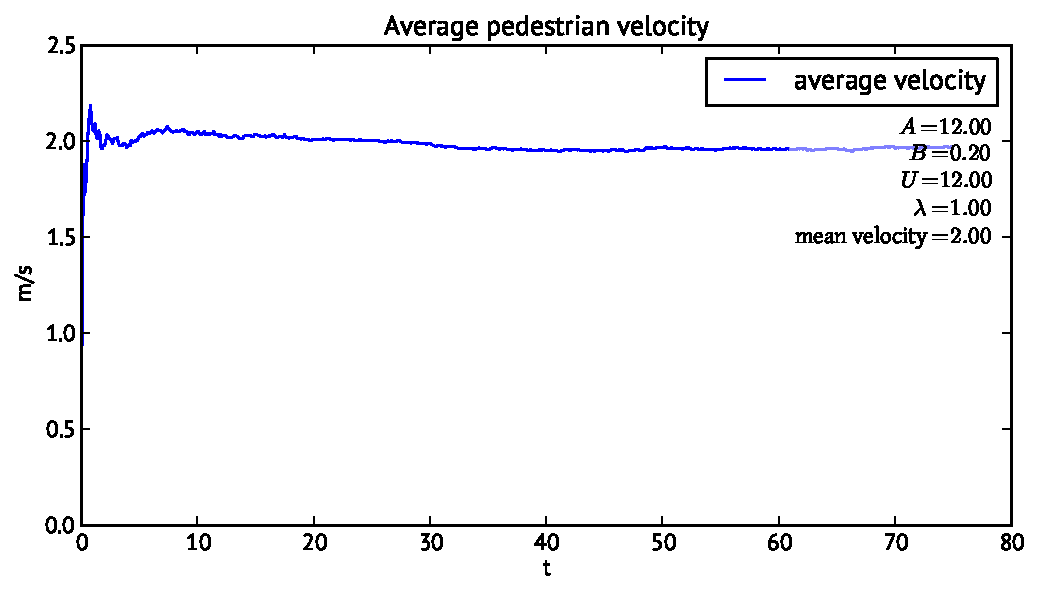
\includegraphics[scale=0.45]{Figures/normalcorridor-velocity.pdf}}
% \subfloat[A graph of the mean velocity of the pedestrian in the corridor with a wide space]{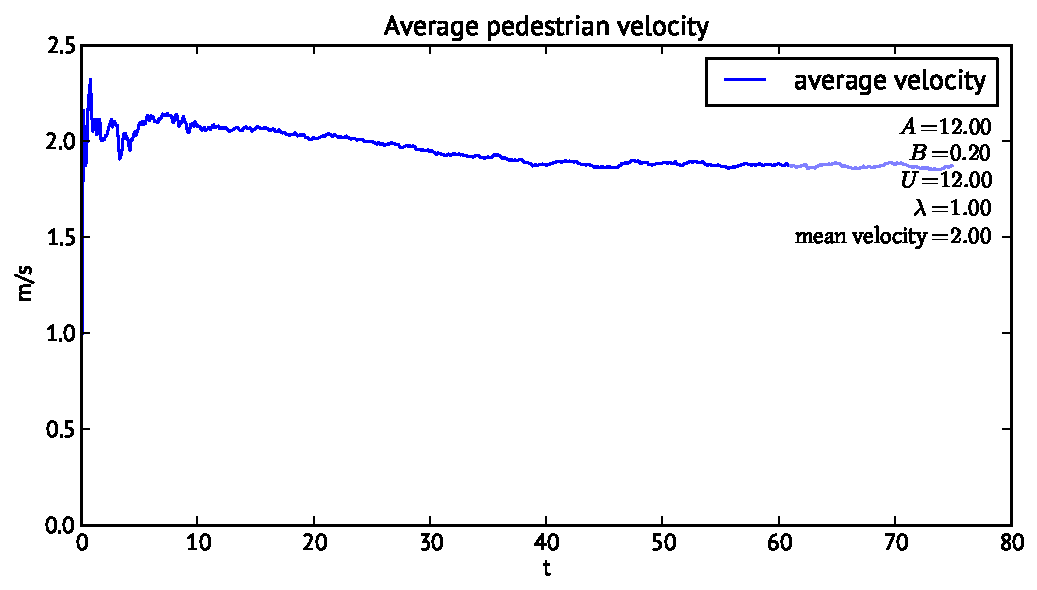
\includegraphics[scale=0.45]{Figures/Widekinkunidirec-velocity.pdf}}\\
% \subfloat[A graph of the flow rate of the pedestrians in the normal corridor]{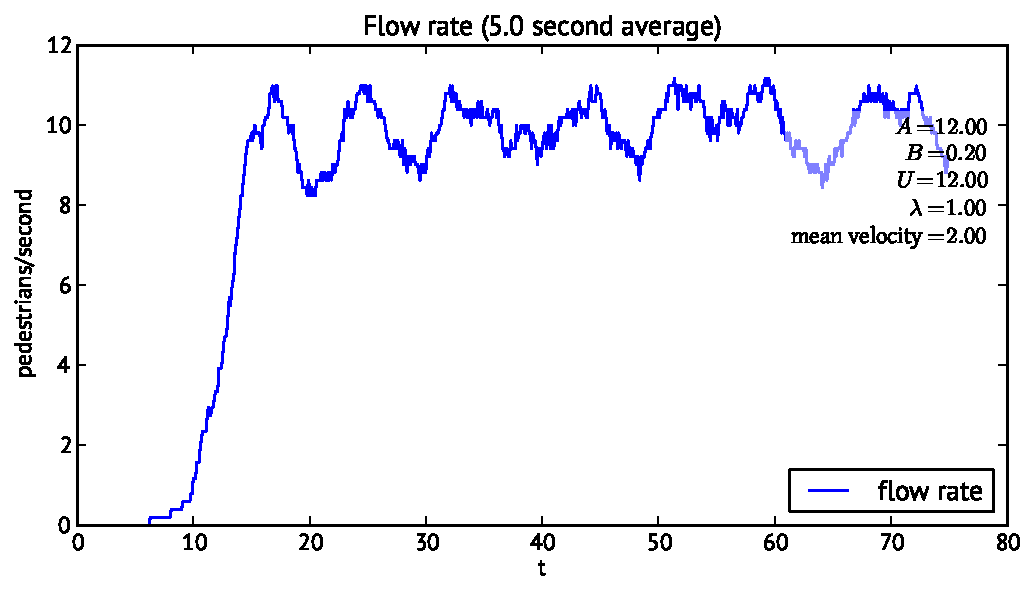
\includegraphics[scale=0.45]{Figures/normalcorridor-flowrate.pdf}}
% \subfloat[A graph of the flowrate in the corridor with the wide space]{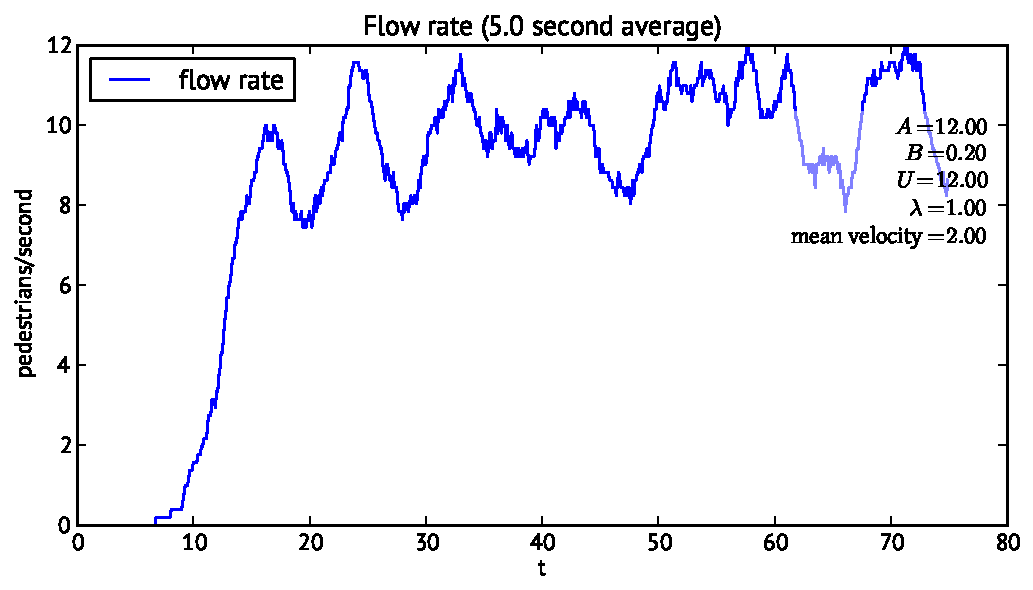
\includegraphics[scale=0.45]{Figures/Widekinkunidirec-flow.pdf}}
% \caption{There is a lowering of the average velocity of the pedestrians due to the bottleneck. We see that there is no consistent lowering of the flowrate due to the bottleneck. What we see is that the flowrate is varying more over time.}
% \label{fig:effect-of-widespace}
% \end{figure}
% 
% % TODO: Add parameters that are varied.
